\documentclass[aspectratio=169,10pt]{beamer}
% Compilar con pdfLaTeX. Compatibilidad con caracteres UTF-8.
\usepackage[utf8]{inputenc}
\usepackage[T1]{fontenc}
\usepackage{lmodern}
\usepackage{amssymb}
\DeclareUnicodeCharacter{2713}{\ensuremath{\checkmark}}
\DeclareUnicodeCharacter{2192}{\ensuremath{\rightarrow}}
\DeclareUnicodeCharacter{2260}{\ensuremath{\neq}}
\DeclareUnicodeCharacter{201C}{``}
\DeclareUnicodeCharacter{201D}{''}
\DeclareUnicodeCharacter{2014}{---}
\usepackage{graphicx}
% Las capturas se encuentran en la carpeta Evidencias/ junto a main.tex.
\graphicspath{{Evidencias/}}
\usepackage{tikz}
\usetikzlibrary{arrows.meta,calc,positioning}
\usepackage{amsmath}
\usepackage[spanish]{babel}
% Tipografía vectorial compatible con pdfLaTeX; preserva el estilo sans serif.
\renewcommand{\sfdefault}{lmss}
\renewcommand{\ttdefault}{lmtt}
\renewcommand{\familydefault}{\sfdefault}
\definecolor{bg}{HTML}{FAF9FE}
\definecolor{white}{HTML}{FFFFFF}
\definecolor{ink}{HTML}{241E41}
\definecolor{muted}{HTML}{746F8B}
\definecolor{accent}{HTML}{7551D6}
\definecolor{wash}{HTML}{EDE7FA}
\definecolor{card}{HTML}{F3F0FB}
\definecolor{linecol}{HTML}{E4DEEF}
\definecolor{blue}{HTML}{347DB7}
\definecolor{teal}{HTML}{21B9A6}
\definecolor{violet2}{HTML}{493578}
\definecolor{deep}{HTML}{191431}
\definecolor{darkviolet}{HTML}{372965}
\definecolor{accentoutline}{HTML}{372B63}
\definecolor{darkline}{HTML}{4A406E}
\definecolor{lilac}{HTML}{D3C6F7}
\definecolor{lightgray}{HTML}{C3BDD5}
\setbeamertemplate{navigation symbols}{}
\setbeamertemplate{footline}{}
\setbeameroption{hide notes}
\begin{document}
\begin{frame}[plain]
\begin{tikzpicture}[remember picture,overlay,x=1cm,y=-1cm]
\begin{scope}[shift={(current page.north west)}]
\path[use as bounding box] (0,0) rectangle (16,9);
\fill[deep] (0,0) rectangle (16,9);
\path[fill=accent, rounded corners=0.00cm] (0.00,0.00) rectangle (0.15,9.00);
\fill[darkviolet] (14.10,7.20) circle (2.00cm);
\fill[accentoutline] (13.90,2.40) circle (2.45cm);
\path[fill=darkviolet, rounded corners=0.17cm] (0.86,0.78) rectangle (5.18,1.36);
\node[anchor=north west,inner sep=0pt,text width=3.89cm,align=left,font={\fontsize{6.43}{8.0}\selectfont\bfseries},text=lilac] at (1.10,0.94) {UTEQ · SOFTWARE · 4.º NIVEL};
\node[anchor=north west,inner sep=0pt,text width=6.90cm,align=left,font={\fontsize{30.82}{38.2}\selectfont\bfseries},text=white] at (0.88,2.03) {TraceCloud};
\node[anchor=north west,inner sep=0pt,text width=7.20cm,align=left,font={\fontsize{15.41}{19.1}\selectfont\bfseries},text=lilac] at (0.90,3.41) {Gestión y trazabilidad};
\node[anchor=north west,inner sep=0pt,text width=7.20cm,align=left,font={\fontsize{14.74}{18.3}\selectfont\bfseries},text=white] at (0.90,4.11) {de requisitos de software};
\draw[draw=teal,line width=0.04cm] (0.93,5.26) -- (7.00,5.26);
\node[anchor=north west,inner sep=0pt,text width=6.80cm,align=left,font={\fontsize{9.38}{11.6}\selectfont\bfseries},text=lilac] at (0.93,5.59) {Exposición GA-SUM-02 · Tema 7};
\node[anchor=north west,inner sep=0pt,text width=7.20cm,align=left,font={\fontsize{8.71}{10.8}\selectfont},text=white] at (0.93,6.18) {Aplicación en Fabro Arriendos};
\node[anchor=north west,inner sep=0pt,text width=7.00cm,align=left,font={\fontsize{6.23}{7.7}\selectfont},text=lightgray] at (0.95,7.75) {Grupo AALM · Quevedo, Ecuador · 2026};
\path[fill=darkviolet, rounded corners=0.18cm] (9.18,1.42) rectangle (15.31,7.17);
\path[fill=white, rounded corners=0.14cm] (9.40,1.67) rectangle (15.04,5.38);
\begin{scope}
\clip[rounded corners=0.09cm] (9.48,1.75) rectangle (14.96,5.30);
\node[anchor=north west,inner sep=0pt] at (9.48,1.75) {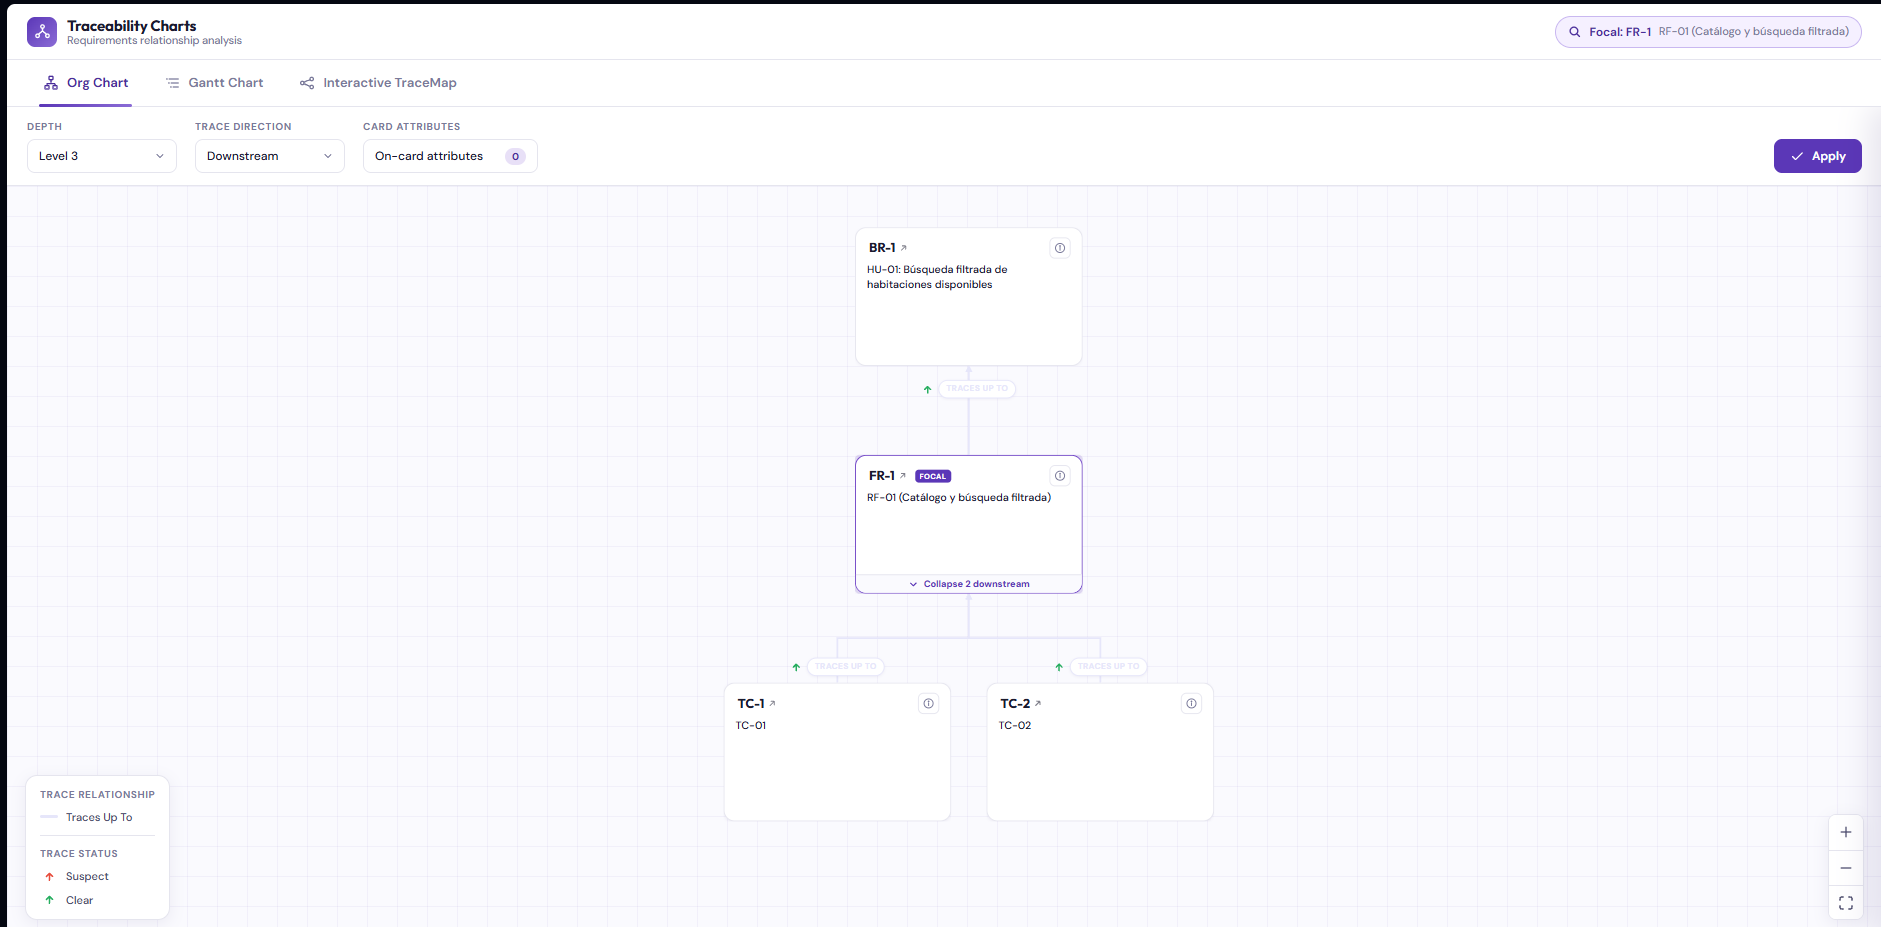
\includegraphics[width=5.48cm,height=3.55cm]{Evidencias/TraceCloud-CAP-04.png}};
\end{scope}
\path[fill=violet2, rounded corners=0.15cm] (9.74,5.63) rectangle (14.69,6.34);
\node[anchor=north west,inner sep=0pt,text width=4.50cm,align=center,font={\fontsize{9.38}{11.6}\selectfont\bfseries},text=white] at (9.95,5.85) {BR-1  →  FR-1  →  TC-1 / TC-2};
\node[anchor=north west,inner sep=0pt,text width=2.90cm,align=center,font={\fontsize{6.37}{7.9}\selectfont\bfseries},text=lilac] at (11.00,6.77) {TRAZABILIDAD};
\draw[draw=darkline,line width=0.01cm] (0.76,8.48) -- (15.30,8.48);
\node[anchor=north west,inner sep=0pt,text width=5.00cm,align=left,font={\fontsize{5.36}{6.6}\selectfont\bfseries},text=lilac] at (0.80,8.59) {UTEQ / ISR-401 / AALM};
\node[anchor=north west,inner sep=0pt,text width=0.50cm,align=right,font={\fontsize{6.03}{7.5}\selectfont\bfseries},text=lilac] at (14.80,8.57) {01};
\end{scope}
\end{tikzpicture}
\note{Presentación: “TraceCloud: gestión y trazabilidad de requisitos”. Este trabajo corresponde a la actividad GA-SUM-02 de Ingeniería de Requerimientos, carrera de Software, cuarto nivel, paralelo A, Universidad Técnica Estatal de Quevedo. Integrantes: Erick Adalberto Alvia Villegas, Angelina Julexy Llerena Abril y Frixon Fernando Moran Pilaguano. Empezaremos con el problema que motiva el uso de herramientas especializadas y después mostraremos la demostración realizada sobre Fabro Arriendos.}
\end{frame}

\begin{frame}[plain]
\begin{tikzpicture}[remember picture,overlay,x=1cm,y=-1cm]
\begin{scope}[shift={(current page.north west)}]
\path[use as bounding box] (0,0) rectangle (16,9);
\fill[bg] (0,0) rectangle (16,9);
\fill[accent] (0,0) rectangle (0.15,9);
\fill[wash] (15.10,0.65) circle (0.80cm);
\node[anchor=north west,inner sep=0pt,text width=12.00cm,align=left,font={\fontsize{6.37}{7.9}\selectfont\bfseries},text=accent] at (0.76,0.46) {02 / FUNDAMENTOS};
\node[anchor=north west,inner sep=0pt,text width=14.50cm,align=left,font={\fontsize{16.42}{20.4}\selectfont\bfseries},text=ink] at (0.76,1.08) {Elicitación, gestión y conocimiento};
\node[anchor=north west,inner sep=0pt,text width=14.10cm,align=left,font={\fontsize{8.17}{10.1}\selectfont},text=muted] at (0.79,1.91) {De las necesidades explícitas o implícitas a requisitos trazables [1]--[3].};
\draw[draw=linecol,line width=0.01cm] (0.77,8.48) -- (15.28,8.48);
\node[anchor=north west,inner sep=0pt,text width=7.00cm,align=left,font={\fontsize{5.16}{6.4}\selectfont\bfseries},text=muted] at (0.78,8.61) {UTEQ  /  ISR-401  /  AALM};
\node[anchor=north west,inner sep=0pt,text width=0.50cm,align=right,font={\fontsize{5.83}{7.2}\selectfont\bfseries},text=muted] at (14.82,8.60) {02};
\path[fill=white, rounded corners=0.20cm] (0.85,2.75) rectangle (5.58,6.28);
\fill[accent] (1.45,3.31) circle (0.36cm);
\node[anchor=north west,inner sep=0pt,text width=0.36cm,align=center,font={\fontsize{6.97}{8.6}\selectfont\bfseries},text=white] at (1.28,3.18) {01};
\node[anchor=north west,inner sep=0pt,text width=4.00cm,align=left,font={\fontsize{15.41}{19.1}\selectfont\bfseries},text=ink] at (1.28,4.02) {Elicitación};
\node[anchor=north west,inner sep=0pt,text width=4.12cm,align=left,font={\fontsize{9.38}{11.6}\selectfont\bfseries},text=accent] at (1.28,4.81) {Descubrir necesidades};
\node[anchor=north west,inner sep=0pt,text width=4.05cm,align=left,font={\fontsize{6.90}{8.6}\selectfont},text=muted] at (1.28,5.40) {Entrevistas y observación};
\path[fill=white, rounded corners=0.20cm] (5.96,2.75) rectangle (10.69,6.28);
\fill[accent] (6.56,3.31) circle (0.36cm);
\node[anchor=north west,inner sep=0pt,text width=0.36cm,align=center,font={\fontsize{6.97}{8.6}\selectfont\bfseries},text=white] at (6.39,3.18) {02};
\node[anchor=north west,inner sep=0pt,text width=4.00cm,align=left,font={\fontsize{15.41}{19.1}\selectfont\bfseries},text=ink] at (6.39,4.02) {Gestión};
\node[anchor=north west,inner sep=0pt,text width=4.12cm,align=left,font={\fontsize{9.38}{11.6}\selectfont\bfseries},text=accent] at (6.39,4.81) {Organizar y controlar};
\node[anchor=north west,inner sep=0pt,text width=4.05cm,align=left,font={\fontsize{6.90}{8.6}\selectfont},text=muted] at (6.39,5.40) {Versiones, estados y cambios};
\path[fill=white, rounded corners=0.20cm] (11.07,2.75) rectangle (15.80,6.28);
\fill[accent] (11.67,3.31) circle (0.36cm);
\node[anchor=north west,inner sep=0pt,text width=0.36cm,align=center,font={\fontsize{6.97}{8.6}\selectfont\bfseries},text=white] at (11.50,3.18) {03};
\node[anchor=north west,inner sep=0pt,text width=4.00cm,align=left,font={\fontsize{15.41}{19.1}\selectfont\bfseries},text=ink] at (11.50,4.02) {Trazabilidad};
\node[anchor=north west,inner sep=0pt,text width=4.12cm,align=left,font={\fontsize{9.38}{11.6}\selectfont\bfseries},text=accent] at (11.50,4.81) {Relacionar elementos};
\node[anchor=north west,inner sep=0pt,text width=4.05cm,align=left,font={\fontsize{6.90}{8.6}\selectfont},text=muted] at (11.50,5.40) {Origen, requisitos y pruebas};
\path[fill=wash, rounded corners=0.15cm] (0.90,6.63) rectangle (7.68,7.67);
\path[fill=wash, rounded corners=0.15cm] (8.05,6.63) rectangle (15.15,7.67);
\node[anchor=north west,inner sep=0pt,text width=6.20cm,align=left,font={\fontsize{8.60}{11.0}\selectfont\bfseries},text=ink] at (1.20,6.83) {Consciente: necesidades expresables};
\node[anchor=north west,inner sep=0pt,text width=6.40cm,align=left,font={\fontsize{8.60}{11.0}\selectfont\bfseries},text=ink] at (8.35,6.83) {Implícito: hábitos y supuestos};
\node[anchor=north west,inner sep=0pt,text width=6.25cm,align=left,font={\fontsize{7.00}{8.7}\selectfont},text=muted] at (1.21,7.27) {Se registran tras su clarificación};
\node[anchor=north west,inner sep=0pt,text width=6.35cm,align=left,font={\fontsize{7.00}{8.7}\selectfont},text=muted] at (8.37,7.27) {Entrevistas y observación para descubrirlos};
\end{scope}
\end{tikzpicture}
\note{El conocimiento puede ser expresable (consciente) o implícito (hábitos, supuestos y rutinas). Las entrevistas, observación o talleres permiten descubrir lo no verbalizado, antes de formular y documentar requisitos. Referencias [1], [2] y [3]. La elicitación reúne actividades para descubrir y comprender necesidades expresadas o implícitas. La gestión mantiene los requisitos organizados, actualizados y bajo control; la trazabilidad documenta relaciones explícitas con orígenes, dependencias y pruebas. TraceCloud se concentra principalmente en almacenar y controlar requisitos que ya han sido formulados. El flujo visual no pretende presentar fases aisladas o rígidamente lineales: en la práctica las actividades pueden iterarse a lo largo del proyecto.}
\end{frame}

\begin{frame}[plain]
\begin{tikzpicture}[remember picture,overlay,x=1cm,y=-1cm]
\begin{scope}[shift={(current page.north west)}]
\path[use as bounding box] (0,0) rectangle (16,9);
\fill[bg] (0,0) rectangle (16,9);
\fill[accent] (0,0) rectangle (0.15,9);
\fill[wash] (15.10,0.65) circle (0.80cm);
\node[anchor=north west,inner sep=0pt,text width=12.00cm,align=left,font={\fontsize{6.37}{7.9}\selectfont\bfseries},text=accent] at (0.76,0.46) {03 / HERRAMIENTA};
\node[anchor=north west,inner sep=0pt,text width=14.50cm,align=left,font={\fontsize{16.42}{20.4}\selectfont\bfseries},text=ink] at (0.76,1.08) {TraceCloud: definición y propósito};
\node[anchor=north west,inner sep=0pt,text width=14.10cm,align=left,font={\fontsize{8.17}{10.1}\selectfont},text=muted] at (0.79,1.91) {Solución al problema de requisitos dispersos en Word y Excel [8].};
\draw[draw=linecol,line width=0.01cm] (0.77,8.48) -- (15.28,8.48);
\node[anchor=north west,inner sep=0pt,text width=7.00cm,align=left,font={\fontsize{5.16}{6.4}\selectfont\bfseries},text=muted] at (0.78,8.61) {UTEQ  /  ISR-401  /  AALM};
\node[anchor=north west,inner sep=0pt,text width=0.50cm,align=right,font={\fontsize{5.83}{7.2}\selectfont\bfseries},text=muted] at (14.82,8.60) {03};
\path[fill=linecol, rounded corners=0.12cm] (0.95,2.84) rectangle (9.48,7.10);
\path[fill=white, rounded corners=0.14cm] (0.79,2.66) rectangle (9.48,7.08);
\begin{scope}
\clip[rounded corners=0.09cm] (0.87,2.74) rectangle (9.40,7.00);
\node[anchor=north west,inner sep=0pt] at (0.87,2.74) {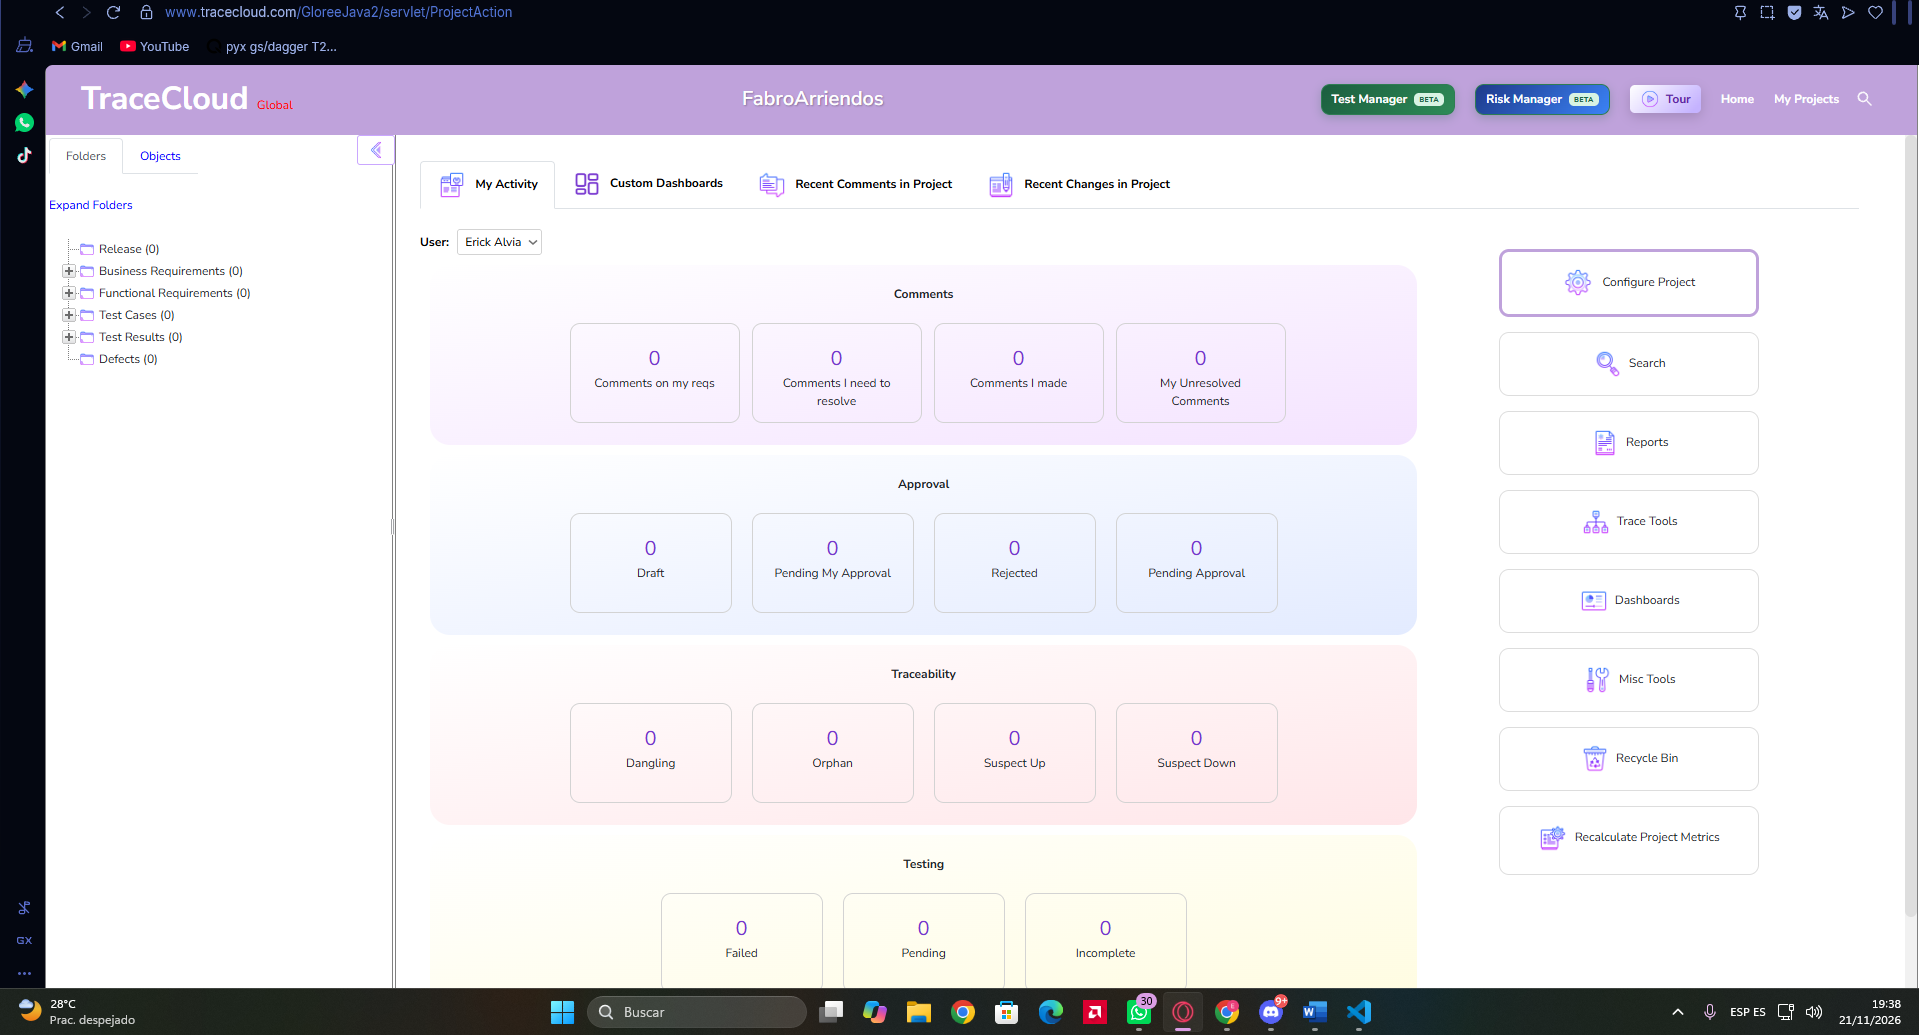
\includegraphics[width=8.53cm,height=4.26cm]{Evidencias/TraceCloud-CAP-01.png}};
\end{scope}
\path[fill=wash, rounded corners=0.20cm] (9.79,2.77) rectangle (15.03,6.96);
\node[anchor=north west,inner sep=0pt,text width=4.50cm,align=left,font={\fontsize{6.70}{8.3}\selectfont\bfseries},text=accent] at (10.20,3.17) {¿QUÉ PERMITE?};
\node[anchor=north west,inner sep=0pt,text width=4.31cm,align=left,font={\fontsize{11.39}{14.1}\selectfont\bfseries},text=ink] at (10.21,3.88) {Definir y organizar};
\draw[draw=linecol,line width=0.01cm] (10.20,4.42) -- (14.61,4.42);
\node[anchor=north west,inner sep=0pt,text width=4.40cm,align=left,font={\fontsize{9.38}{11.6}\selectfont\bfseries},text=ink] at (10.21,4.70) {Controlar versiones y aprobación};
\draw[draw=linecol,line width=0.01cm] (10.20,5.32) -- (14.61,5.32);
\node[anchor=north west,inner sep=0pt,text width=4.25cm,align=left,font={\fontsize{11.39}{14.1}\selectfont\bfseries},text=ink] at (10.21,5.69) {Rastrear relaciones};
\node[anchor=north west,inner sep=0pt,text width=8.00cm,align=left,font={\fontsize{6.10}{7.6}\selectfont},text=muted] at (0.91,7.21) {Problema: documentos aislados; respuesta: repositorio con vínculos [8].};
\end{scope}
\end{tikzpicture}
\note{El problema introductorio de requisitos dispersos en Word/Excel se ha integrado en esta lámina para evitar redundancias. La documentación del fabricante [8] indica centralización y trazabilidad. TraceCloud se presenta en su documento técnico como una herramienta para definir, aprobar, controlar y dar seguimiento a requisitos. Admite diferentes tipos y atributos, gestión de versiones, permisos y visualizaciones de trazabilidad. El documento del fabricante de 2020 describe opciones de uso en la nube o infraestructura propia; algunas capacidades pueden haber cambiado. Se muestra el panel real del proyecto FabroArriendos capturado por el equipo.}
\end{frame}

\begin{frame}[plain]
\begin{tikzpicture}[remember picture,overlay,x=1cm,y=-1cm]
\begin{scope}[shift={(current page.north west)}]
\path[use as bounding box] (0,0) rectangle (16,9);
\fill[bg] (0,0) rectangle (16,9);
\fill[accent] (0,0) rectangle (0.15,9);
\fill[wash] (15.10,0.65) circle (0.80cm);
\node[anchor=north west,inner sep=0pt,text width=12.00cm,align=left,font={\fontsize{6.37}{7.9}\selectfont\bfseries},text=accent] at (0.76,0.46) {03 / HERRAMIENTA};
\node[anchor=north west,inner sep=0pt,text width=14.50cm,align=left,font={\fontsize{16.42}{20.4}\selectfont\bfseries},text=ink] at (0.76,1.08) {Funciones para controlar requisitos};
\node[anchor=north west,inner sep=0pt,text width=14.10cm,align=left,font={\fontsize{8.17}{10.1}\selectfont},text=muted] at (0.79,1.91) {Árbol, matriz, Org Chart, baselines y alertas SUSPECT [8].};
\draw[draw=linecol,line width=0.01cm] (0.77,8.48) -- (15.28,8.48);
\node[anchor=north west,inner sep=0pt,text width=7.00cm,align=left,font={\fontsize{5.16}{6.4}\selectfont\bfseries},text=muted] at (0.78,8.61) {UTEQ  /  ISR-401  /  AALM};
\node[anchor=north west,inner sep=0pt,text width=0.50cm,align=right,font={\fontsize{5.83}{7.2}\selectfont\bfseries},text=muted] at (14.82,8.60) {04};
\path[fill=violet2, rounded corners=0.21cm] (0.87,2.65) rectangle (6.43,7.13);
\node[anchor=north west,inner sep=0pt,text width=4.70cm,align=left,font={\fontsize{6.70}{8.3}\selectfont\bfseries},text=lilac] at (1.19,3.03) {FUNCIÓN DESTACADA};
\node[anchor=north west,inner sep=0pt,text width=4.95cm,align=left,font={\fontsize{18.76}{23.3}\selectfont\bfseries},text=white] at (1.17,3.74) {SUSPECT};
\node[anchor=north west,inner sep=0pt,text width=4.95cm,align=left,font={\fontsize{18.76}{23.3}\selectfont\bfseries},text=white] at (1.17,4.43) {TRACES};
\node[anchor=north west,inner sep=0pt,text width=4.79cm,align=left,font={\fontsize{9.38}{11.6}\selectfont},text=white] at (1.19,5.46) {Marca relaciones que requieren revisión tras modificar un requisito.};
\path[fill=white, rounded corners=0.19cm] (6.77,2.68) rectangle (10.68,4.70);
\fill[accent] (7.26,3.17) circle (0.22cm);
\node[anchor=north west,inner sep=0pt,text width=3.40cm,align=left,font={\fontsize{10.92}{13.5}\selectfont\bfseries},text=ink] at (7.07,3.62) {Trace Tree};
\node[anchor=north west,inner sep=0pt,text width=3.35cm,align=left,font={\fontsize{7.37}{9.1}\selectfont},text=muted] at (7.08,4.19) {Árbol de relaciones};
\path[fill=white, rounded corners=0.19cm] (11.03,2.68) rectangle (14.94,4.70);
\fill[accent] (11.52,3.17) circle (0.22cm);
\node[anchor=north west,inner sep=0pt,text width=3.40cm,align=left,font={\fontsize{10.92}{13.5}\selectfont\bfseries},text=ink] at (11.33,3.62) {Trace Matrix};
\node[anchor=north west,inner sep=0pt,text width=3.35cm,align=left,font={\fontsize{7.37}{9.1}\selectfont},text=muted] at (11.34,4.19) {Matriz de trazas};
\path[fill=white, rounded corners=0.19cm] (6.77,4.96) rectangle (10.68,6.98);
\fill[accent] (7.26,5.45) circle (0.22cm);
\node[anchor=north west,inner sep=0pt,text width=3.40cm,align=left,font={\fontsize{10.92}{13.5}\selectfont\bfseries},text=ink] at (7.07,5.90) {Trace Org Chart};
\node[anchor=north west,inner sep=0pt,text width=3.35cm,align=left,font={\fontsize{7.37}{9.1}\selectfont},text=muted] at (7.08,6.47) {Diagrama de trazabilidad};
\path[fill=white, rounded corners=0.19cm] (11.03,4.96) rectangle (14.94,6.98);
\fill[accent] (11.52,5.45) circle (0.22cm);
\node[anchor=north west,inner sep=0pt,text width=3.40cm,align=left,font={\fontsize{10.92}{13.5}\selectfont\bfseries},text=ink] at (11.33,5.90) {Baselines};
\node[anchor=north west,inner sep=0pt,text width=3.35cm,align=left,font={\fontsize{7.37}{9.1}\selectfont},text=muted] at (11.34,6.47) {Líneas base};
\node[anchor=north west,inner sep=0pt,text width=14.10cm,align=left,font={\fontsize{6.45}{8.5}\selectfont},text=muted] at (0.98,7.56) {IA generativa y LLM: líneas de apoyo distintas de la gestión demostrada [4], [5].};
\end{scope}
\end{tikzpicture}
\note{Las publicaciones [4] y [5] estudian IA generativa y grandes modelos de lenguaje en ingeniería de requisitos, un ámbito distinto de las funciones específicas documentadas y ensayadas de TraceCloud. No afirmar que las funciones presentadas dependen de IA generativa. Entre las funcionalidades documentadas se encuentran las vistas Trace Tree, Trace Matrix y Trace Org Chart, así como las líneas base, las aprobaciones y la identificación de requisitos sin trazas ascendentes u horizontales. La característica que el equipo puso a prueba fue la alerta Suspect: después de modificar un requisito vinculado, la herramienta marca una relación que requiere nueva revisión. La alerta no implica por sí sola que el requisito sea inválido ni que la plataforma haya corregido el cambio automáticamente.}
\end{frame}

\begin{frame}[plain]
\begin{tikzpicture}[remember picture,overlay,x=1cm,y=-1cm]
\begin{scope}[shift={(current page.north west)}]
\path[use as bounding box] (0,0) rectangle (16,9);
\fill[bg] (0,0) rectangle (16,9);
\fill[accent] (0,0) rectangle (0.15,9);
\fill[wash] (15.10,0.65) circle (0.80cm);
\node[anchor=north west,inner sep=0pt,text width=12.00cm,align=left,font={\fontsize{6.37}{7.9}\selectfont\bfseries},text=accent] at (0.76,0.46) {04 / DECISIÓN DE USO};
\node[anchor=north west,inner sep=0pt,text width=14.50cm,align=left,font={\fontsize{16.42}{20.4}\selectfont\bfseries},text=ink] at (0.76,1.08) {¿Cuándo conviene utilizarla?};
\node[anchor=north west,inner sep=0pt,text width=14.10cm,align=left,font={\fontsize{8.17}{10.1}\selectfont},text=muted] at (0.79,1.91) {La adopción depende de escala, trazabilidad y control [1], [6], [8].};
\draw[draw=linecol,line width=0.01cm] (0.77,8.48) -- (15.28,8.48);
\node[anchor=north west,inner sep=0pt,text width=7.00cm,align=left,font={\fontsize{5.16}{6.4}\selectfont\bfseries},text=muted] at (0.78,8.61) {UTEQ  /  ISR-401  /  AALM};
\node[anchor=north west,inner sep=0pt,text width=0.50cm,align=right,font={\fontsize{5.83}{7.2}\selectfont\bfseries},text=muted] at (14.82,8.60) {05};
\path[fill=white, rounded corners=0.18cm] (0.86,2.68) rectangle (7.96,6.91);
\node[anchor=north west,inner sep=0pt,text width=6.00cm,align=left,font={\fontsize{7.77}{9.6}\selectfont\bfseries},text=teal] at (1.25,3.04) {CONVIENE};
\fill[teal] (1.43,3.84) circle (0.14cm);
\node[anchor=north west,inner sep=0pt,text width=0.30cm,align=center,font={\fontsize{6.70}{8.3}\selectfont\bfseries},text=white] at (1.28,3.72) {✓};
\node[anchor=north west,inner sep=0pt,text width=5.75cm,align=left,font={\fontsize{9.38}{11.6}\selectfont},text=ink] at (1.82,3.69) {Requisitos numerosos o dispersos};
\fill[teal] (1.43,4.52) circle (0.14cm);
\node[anchor=north west,inner sep=0pt,text width=0.30cm,align=center,font={\fontsize{6.70}{8.3}\selectfont\bfseries},text=white] at (1.28,4.40) {✓};
\node[anchor=north west,inner sep=0pt,text width=5.75cm,align=left,font={\fontsize{9.38}{11.6}\selectfont},text=ink] at (1.82,4.37) {Cambios con dependencias};
\fill[teal] (1.43,5.20) circle (0.14cm);
\node[anchor=north west,inner sep=0pt,text width=0.30cm,align=center,font={\fontsize{6.70}{8.3}\selectfont\bfseries},text=white] at (1.28,5.08) {✓};
\node[anchor=north west,inner sep=0pt,text width=5.75cm,align=left,font={\fontsize{9.38}{11.6}\selectfont},text=ink] at (1.82,5.05) {Roles y permisos diferenciados};
\fill[teal] (1.43,5.88) circle (0.14cm);
\node[anchor=north west,inner sep=0pt,text width=0.30cm,align=center,font={\fontsize{6.70}{8.3}\selectfont\bfseries},text=white] at (1.28,5.76) {✓};
\node[anchor=north west,inner sep=0pt,text width=5.75cm,align=left,font={\fontsize{9.38}{11.6}\selectfont},text=ink] at (1.82,5.73) {Aprobaciones y líneas base};
\path[fill=wash, rounded corners=0.18cm] (8.32,2.68) rectangle (15.16,6.91);
\node[anchor=north west,inner sep=0pt,text width=6.00cm,align=left,font={\fontsize{7.77}{9.6}\selectfont\bfseries},text=accent] at (8.68,3.04) {NO ES PRIORITARIA};
\fill[accent] (8.84,3.87) circle (0.14cm);
\node[anchor=north west,inner sep=0pt,text width=0.20cm,align=center,font={\fontsize{6.70}{8.3}\selectfont\bfseries},text=white] at (8.79,3.76) {!};
\node[anchor=north west,inner sep=0pt,text width=5.32cm,align=left,font={\fontsize{8.78}{10.9}\selectfont},text=ink] at (9.25,3.72) {Proyectos muy pequeños};
\fill[accent] (8.84,4.69) circle (0.14cm);
\node[anchor=north west,inner sep=0pt,text width=0.20cm,align=center,font={\fontsize{6.70}{8.3}\selectfont\bfseries},text=white] at (8.79,4.58) {!};
\node[anchor=north west,inner sep=0pt,text width=5.32cm,align=left,font={\fontsize{8.78}{10.9}\selectfont},text=ink] at (9.25,4.54) {Descubrimiento inicial};
\fill[accent] (8.84,5.51) circle (0.14cm);
\node[anchor=north west,inner sep=0pt,text width=0.20cm,align=center,font={\fontsize{6.70}{8.3}\selectfont\bfseries},text=white] at (8.79,5.40) {!};
\node[anchor=north west,inner sep=0pt,text width=5.32cm,align=left,font={\fontsize{8.78}{10.9}\selectfont},text=ink] at (9.25,5.36) {ReqIF como requisito obligatorio};
\node[anchor=north west,inner sep=0pt,text width=12.50cm,align=left,font={\fontsize{6.50}{8.1}\selectfont},text=muted] at (0.92,7.40) {ReqIF: compatibilidad no documentada en la fuente consultada.};
\end{scope}
\end{tikzpicture}
\note{TraceCloud resulta apropiada cuando un proyecto maneja numerosos requisitos dispersos, necesita trazabilidad multinivel y requiere control de cambios o aprobación formal. En proyectos cortos con muy pocos requisitos, el esfuerzo de configuración puede resultar excesivo. Tampoco es sustituto de entrevistas ni de otras técnicas de descubrimiento. El informe no encontró declaración de compatibilidad con ReqIF en la documentación revisada, por lo que no debe asegurarse que ese formato esté soportado. Es una consideración documental, no una prueba de incompatibilidad absoluta.}
\end{frame}

\begin{frame}[plain]
\begin{tikzpicture}[remember picture,overlay,x=1cm,y=-1cm]
\begin{scope}[shift={(current page.north west)}]
\path[use as bounding box] (0,0) rectangle (16,9);
\fill[bg] (0,0) rectangle (16,9);
\fill[accent] (0,0) rectangle (0.15,9);
\fill[wash] (15.10,0.65) circle (0.80cm);
\node[anchor=north west,inner sep=0pt,text width=12.00cm,align=left,font={\fontsize{6.37}{7.9}\selectfont\bfseries},text=accent] at (0.76,0.46) {05 / PROCEDIMIENTO};
\node[anchor=north west,inner sep=0pt,text width=14.50cm,align=left,font={\fontsize{16.42}{20.4}\selectfont\bfseries},text=ink] at (0.76,1.08) {Cinco pasos para aplicarla};
\node[anchor=north west,inner sep=0pt,text width=14.10cm,align=left,font={\fontsize{8.17}{10.1}\selectfont},text=muted] at (0.79,1.91) {Procedimiento documentado y aplicado en el caso [8].};
\draw[draw=linecol,line width=0.01cm] (0.77,8.48) -- (15.28,8.48);
\node[anchor=north west,inner sep=0pt,text width=7.00cm,align=left,font={\fontsize{5.16}{6.4}\selectfont\bfseries},text=muted] at (0.78,8.61) {UTEQ  /  ISR-401  /  AALM};
\node[anchor=north west,inner sep=0pt,text width=0.50cm,align=right,font={\fontsize{5.83}{7.2}\selectfont\bfseries},text=muted] at (14.82,8.60) {06};
\path[fill=white, rounded corners=0.19cm] (0.77,3.27) rectangle (3.63,5.96);
\fill[accent] (2.19,3.79) circle (0.42cm);
\node[anchor=north west,inner sep=0pt,text width=0.52cm,align=center,font={\fontsize{9.04}{11.2}\selectfont\bfseries},text=white] at (1.93,3.62) {01};
\node[anchor=north west,inner sep=0pt,text width=2.48cm,align=center,font={\fontsize{10.18}{12.6}\selectfont\bfseries},text=ink] at (0.95,4.55) {Crear};
\node[anchor=north west,inner sep=0pt,text width=2.48cm,align=center,font={\fontsize{7.17}{8.9}\selectfont},text=muted] at (0.96,5.17) {Proyecto y plantilla};
\draw[draw=accent,line width=0.04cm,-Latex] (3.63,4.62) -- (3.84,4.62);
\path[fill=white, rounded corners=0.19cm] (3.89,3.27) rectangle (6.75,5.96);
\fill[accent] (5.31,3.79) circle (0.42cm);
\node[anchor=north west,inner sep=0pt,text width=0.52cm,align=center,font={\fontsize{9.04}{11.2}\selectfont\bfseries},text=white] at (5.05,3.62) {02};
\node[anchor=north west,inner sep=0pt,text width=2.48cm,align=center,font={\fontsize{10.18}{12.6}\selectfont\bfseries},text=ink] at (4.07,4.55) {Configurar};
\node[anchor=north west,inner sep=0pt,text width=2.48cm,align=center,font={\fontsize{7.17}{8.9}\selectfont},text=muted] at (4.08,5.17) {Carpetas y roles};
\draw[draw=accent,line width=0.04cm,-Latex] (6.75,4.62) -- (6.96,4.62);
\path[fill=white, rounded corners=0.19cm] (7.01,3.27) rectangle (9.87,5.96);
\fill[accent] (8.43,3.79) circle (0.42cm);
\node[anchor=north west,inner sep=0pt,text width=0.52cm,align=center,font={\fontsize{9.04}{11.2}\selectfont\bfseries},text=white] at (8.17,3.62) {03};
\node[anchor=north west,inner sep=0pt,text width=2.48cm,align=center,font={\fontsize{10.18}{12.6}\selectfont\bfseries},text=ink] at (7.19,4.55) {Registrar};
\node[anchor=north west,inner sep=0pt,text width=2.48cm,align=center,font={\fontsize{7.17}{8.9}\selectfont},text=muted] at (7.20,5.17) {BR, FR y pruebas};
\draw[draw=accent,line width=0.04cm,-Latex] (9.87,4.62) -- (10.08,4.62);
\path[fill=white, rounded corners=0.19cm] (10.13,3.27) rectangle (12.99,5.96);
\fill[accent] (11.55,3.79) circle (0.42cm);
\node[anchor=north west,inner sep=0pt,text width=0.52cm,align=center,font={\fontsize{9.04}{11.2}\selectfont\bfseries},text=white] at (11.29,3.62) {04};
\node[anchor=north west,inner sep=0pt,text width=2.48cm,align=center,font={\fontsize{10.18}{12.6}\selectfont\bfseries},text=ink] at (10.31,4.55) {Relacionar};
\node[anchor=north west,inner sep=0pt,text width=2.48cm,align=center,font={\fontsize{7.17}{8.9}\selectfont},text=muted] at (10.32,5.17) {Trazas entre niveles};
\draw[draw=accent,line width=0.04cm,-Latex] (12.99,4.62) -- (13.20,4.62);
\path[fill=white, rounded corners=0.19cm] (13.25,3.27) rectangle (16.11,5.96);
\fill[accent] (14.67,3.79) circle (0.42cm);
\node[anchor=north west,inner sep=0pt,text width=0.52cm,align=center,font={\fontsize{9.04}{11.2}\selectfont\bfseries},text=white] at (14.41,3.62) {05};
\node[anchor=north west,inner sep=0pt,text width=2.48cm,align=center,font={\fontsize{10.18}{12.6}\selectfont\bfseries},text=ink] at (13.43,4.55) {Revisar};
\node[anchor=north west,inner sep=0pt,text width=2.48cm,align=center,font={\fontsize{7.17}{8.9}\selectfont},text=muted] at (13.44,5.17) {Cambios y reportes};
\node[anchor=north west,inner sep=0pt,text width=10.60cm,align=center,font={\fontsize{9.38}{11.6}\selectfont\bfseries},text=accent] at (2.80,6.94) {Del requisito registrado al impacto revisable};
\end{scope}
\end{tikzpicture}
\note{La secuencia reproducible indicada en el informe comienza creando un proyecto con la plantilla Generic. Después se ajustan la estructura de carpetas, atributos y permisos. Se registran o importan requisitos de negocio, funcionales y casos de prueba, se establecen relaciones entre ellos y se revisan los cambios mediante vistas de trazabilidad, reportes y paneles. En el caso práctico el equipo creó FabroArriendos, registró BR y FR, trazó FR-1 con BR-1 y dos casos de prueba y provocó una alerta Suspect.}
\end{frame}

\begin{frame}[plain]
\begin{tikzpicture}[remember picture,overlay,x=1cm,y=-1cm]
\begin{scope}[shift={(current page.north west)}]
\path[use as bounding box] (0,0) rectangle (16,9);
\fill[bg] (0,0) rectangle (16,9);
\fill[accent] (0,0) rectangle (0.15,9);
\fill[wash] (15.10,0.65) circle (0.80cm);
\node[anchor=north west,inner sep=0pt,text width=12.00cm,align=left,font={\fontsize{6.37}{7.9}\selectfont\bfseries},text=accent] at (0.76,0.46) {06 / ANÁLISIS CRÍTICO};
\node[anchor=north west,inner sep=0pt,text width=14.50cm,align=left,font={\fontsize{16.42}{20.4}\selectfont\bfseries},text=ink] at (0.76,1.08) {TraceCloud frente a Jira};
\node[anchor=north west,inner sep=0pt,text width=14.10cm,align=left,font={\fontsize{8.17}{10.1}\selectfont},text=muted] at (0.79,1.91) {Evaluación de capacidades documentadas, no de versiones actuales [7], [8].};
\draw[draw=linecol,line width=0.01cm] (0.77,8.48) -- (15.28,8.48);
\node[anchor=north west,inner sep=0pt,text width=7.00cm,align=left,font={\fontsize{5.16}{6.4}\selectfont\bfseries},text=muted] at (0.78,8.61) {UTEQ  /  ISR-401  /  AALM};
\node[anchor=north west,inner sep=0pt,text width=0.50cm,align=right,font={\fontsize{5.83}{7.2}\selectfont\bfseries},text=muted] at (14.82,8.60) {07};
\path[fill=wash, rounded corners=0.17cm] (0.85,2.61) rectangle (7.82,7.39);
\fill[accent] (1.58,3.30) circle (0.38cm);
\node[anchor=north west,inner sep=0pt,text width=0.34cm,align=center,font={\fontsize{12.06}{15.0}\selectfont\bfseries},text=white] at (1.41,3.14) {T};
\node[anchor=north west,inner sep=0pt,text width=5.10cm,align=left,font={\fontsize{14.74}{18.3}\selectfont\bfseries},text=ink] at (2.17,3.08) {TraceCloud};
\path[fill=white, rounded corners=0.17cm] (8.12,2.61) rectangle (15.09,7.39);
\fill[blue] (8.85,3.30) circle (0.38cm);
\node[anchor=north west,inner sep=0pt,text width=0.34cm,align=center,font={\fontsize{12.06}{15.0}\selectfont\bfseries},text=white] at (8.68,3.14) {J};
\node[anchor=north west,inner sep=0pt,text width=5.10cm,align=left,font={\fontsize{14.74}{18.3}\selectfont\bfseries},text=ink] at (9.44,3.08) {Jira};
\node[anchor=north west,inner sep=0pt,text width=6.00cm,align=left,font={\fontsize{6.43}{8.0}\selectfont\bfseries},text=accent] at (1.34,3.94) {PROPÓSITO};
\node[anchor=north west,inner sep=0pt,text width=6.00cm,align=left,font={\fontsize{9.25}{11.5}\selectfont\bfseries},text=ink] at (1.34,4.26) {Gestión de requisitos};
\draw[draw=linecol,line width=0.01cm] (1.33,4.76) -- (7.31,4.76);
\node[anchor=north west,inner sep=0pt,text width=6.00cm,align=left,font={\fontsize{6.43}{8.0}\selectfont\bfseries},text=accent] at (8.61,3.94) {PROPÓSITO};
\node[anchor=north west,inner sep=0pt,text width=6.00cm,align=left,font={\fontsize{9.25}{11.5}\selectfont\bfseries},text=ink] at (8.61,4.26) {Gestión de proyectos};
\draw[draw=linecol,line width=0.01cm] (8.60,4.76) -- (14.58,4.76);
\node[anchor=north west,inner sep=0pt,text width=6.00cm,align=left,font={\fontsize{6.43}{8.0}\selectfont\bfseries},text=accent] at (1.34,4.94) {TRAZABILIDAD};
\node[anchor=north west,inner sep=0pt,text width=6.00cm,align=left,font={\fontsize{9.25}{11.5}\selectfont\bfseries},text=ink] at (1.34,5.26) {Árbol, matriz y Org Chart};
\draw[draw=linecol,line width=0.01cm] (1.33,5.76) -- (7.31,5.76);
\node[anchor=north west,inner sep=0pt,text width=6.00cm,align=left,font={\fontsize{6.43}{8.0}\selectfont\bfseries},text=accent] at (8.61,4.94) {TRAZABILIDAD};
\node[anchor=north west,inner sep=0pt,text width=6.00cm,align=left,font={\fontsize{9.25}{11.5}\selectfont\bfseries},text=ink] at (8.61,5.26) {Soporte completo evaluado};
\draw[draw=linecol,line width=0.01cm] (8.60,5.76) -- (14.58,5.76);
\node[anchor=north west,inner sep=0pt,text width=6.00cm,align=left,font={\fontsize{6.43}{8.0}\selectfont\bfseries},text=accent] at (1.34,5.94) {ALCANCE};
\node[anchor=north west,inner sep=0pt,text width=6.00cm,align=left,font={\fontsize{9.25}{11.5}\selectfont\bfseries},text=ink] at (1.34,6.26) {No cubre todo el ciclo};
\node[anchor=north west,inner sep=0pt,text width=6.00cm,align=left,font={\fontsize{6.43}{8.0}\selectfont\bfseries},text=accent] at (8.61,5.94) {ALCANCE};
\node[anchor=north west,inner sep=0pt,text width=6.00cm,align=left,font={\fontsize{9.25}{11.5}\selectfont\bfseries},text=ink] at (8.61,6.26) {Otras funciones: soporte parcial};
\node[anchor=north west,inner sep=0pt,text width=14.70cm,align=left,font={\fontsize{6.57}{8.1}\selectfont},text=muted] at (1.01,7.65) {Criterio: TraceCloud, control formal de requisitos; Jira, gestión de tareas [7], [8].};
\end{scope}
\end{tikzpicture}
\note{Interpretación aplicable al caso: TraceCloud destaca por versiones, aprobaciones y representaciones dedicadas a trazas, y Jira por el seguimiento de trabajo. No se debe suponer superioridad universal ni generalizar la evaluación de una versión a todas las versiones. Jira se orienta principalmente a la gestión de proyectos. TraceCloud se presenta como herramienta especializada en requisitos y trazabilidad. Rozenberga y Kirikova evaluaron funcionalidades de Jira y aplicaciones de su Marketplace, incluida TraceCloud. La evaluación encontró que ninguna de las aplicaciones analizadas cubría por sí sola todo el ciclo de gestión de requisitos. Para Jira se reconoció soporte completo en las funciones de trazabilidad evaluadas, con cobertura parcial en múltiples otras áreas. La comparación de la diapositiva resume el informe; no es una medición actualizada de versiones comerciales.}
\end{frame}

\begin{frame}[plain]
\begin{tikzpicture}[remember picture,overlay,x=1cm,y=-1cm]
\begin{scope}[shift={(current page.north west)}]
\path[use as bounding box] (0,0) rectangle (16,9);
\fill[bg] (0,0) rectangle (16,9);
\fill[accent] (0,0) rectangle (0.15,9);
\fill[wash] (15.10,0.65) circle (0.80cm);
\node[anchor=north west,inner sep=0pt,text width=12.00cm,align=left,font={\fontsize{6.37}{7.9}\selectfont\bfseries},text=accent] at (0.76,0.46) {07 / CASO PRÁCTICO};
\node[anchor=north west,inner sep=0pt,text width=14.50cm,align=left,font={\fontsize{16.42}{20.4}\selectfont\bfseries},text=ink] at (0.76,1.08) {Fabro Arriendos: caso de estudio};
\node[anchor=north west,inner sep=0pt,text width=14.10cm,align=left,font={\fontsize{8.17}{10.1}\selectfont},text=muted] at (0.79,1.91) {Gestión de arriendos para estudiantes y propietarios de Quevedo.};
\draw[draw=linecol,line width=0.01cm] (0.77,8.48) -- (15.28,8.48);
\node[anchor=north west,inner sep=0pt,text width=7.00cm,align=left,font={\fontsize{5.16}{6.4}\selectfont\bfseries},text=muted] at (0.78,8.61) {UTEQ  /  ISR-401  /  AALM};
\node[anchor=north west,inner sep=0pt,text width=0.50cm,align=right,font={\fontsize{5.83}{7.2}\selectfont\bfseries},text=muted] at (14.82,8.60) {08};
\path[fill=white, rounded corners=0.20cm] (0.86,2.72) rectangle (5.61,6.60);
\fill[accent] (1.54,3.37) circle (0.40cm);
\node[anchor=north west,inner sep=0pt,text width=0.27cm,align=center,font={\fontsize{10.72}{13.3}\selectfont\bfseries},text=white] at (1.40,3.17) {1};
\node[anchor=north west,inner sep=0pt,text width=4.20cm,align=left,font={\fontsize{8.38}{10.4}\selectfont\bfseries},text=accent] at (1.28,4.00) {ESTUDIANTE};
\fill[teal] (1.39,4.66) circle (0.05cm);
\node[anchor=north west,inner sep=0pt,text width=3.60cm,align=left,font={\fontsize{7.50}{9.3}\selectfont},text=ink] at (1.62,4.50) {Buscar habitaciones};
\fill[teal] (1.39,5.23) circle (0.05cm);
\node[anchor=north west,inner sep=0pt,text width=3.60cm,align=left,font={\fontsize{7.50}{9.3}\selectfont},text=ink] at (1.62,5.07) {Consultar reglas y precios};
\fill[teal] (1.39,5.80) circle (0.05cm);
\node[anchor=north west,inner sep=0pt,text width=3.60cm,align=left,font={\fontsize{7.50}{9.3}\selectfont},text=ink] at (1.62,5.64) {Reportar incidencias};
\path[fill=white, rounded corners=0.20cm] (5.96,2.72) rectangle (10.71,6.60);
\fill[accent] (6.64,3.37) circle (0.40cm);
\node[anchor=north west,inner sep=0pt,text width=0.27cm,align=center,font={\fontsize{10.72}{13.3}\selectfont\bfseries},text=white] at (6.50,3.17) {2};
\node[anchor=north west,inner sep=0pt,text width=4.20cm,align=left,font={\fontsize{8.38}{10.4}\selectfont\bfseries},text=accent] at (6.38,4.00) {PROPIETARIO};
\fill[teal] (6.49,4.66) circle (0.05cm);
\node[anchor=north west,inner sep=0pt,text width=3.60cm,align=left,font={\fontsize{7.50}{9.3}\selectfont},text=ink] at (6.72,4.50) {Administrar habitaciones};
\fill[teal] (6.49,5.23) circle (0.05cm);
\node[anchor=north west,inner sep=0pt,text width=3.60cm,align=left,font={\fontsize{7.50}{9.3}\selectfont},text=ink] at (6.72,5.07) {Registrar pagos};
\fill[teal] (6.49,5.80) circle (0.05cm);
\node[anchor=north west,inner sep=0pt,text width=3.60cm,align=left,font={\fontsize{7.50}{9.3}\selectfont},text=ink] at (6.72,5.64) {Gestionar mantenimiento};
\path[fill=white, rounded corners=0.20cm] (11.06,2.72) rectangle (15.81,6.60);
\fill[accent] (11.74,3.37) circle (0.40cm);
\node[anchor=north west,inner sep=0pt,text width=0.27cm,align=center,font={\fontsize{10.72}{13.3}\selectfont\bfseries},text=white] at (11.60,3.17) {3};
\node[anchor=north west,inner sep=0pt,text width=4.20cm,align=left,font={\fontsize{8.38}{10.4}\selectfont\bfseries},text=accent] at (11.48,4.00) {ADMINISTRADOR};
\fill[teal] (11.59,4.66) circle (0.05cm);
\node[anchor=north west,inner sep=0pt,text width=3.60cm,align=left,font={\fontsize{7.50}{9.3}\selectfont},text=ink] at (11.82,4.50) {Verificar publicaciones};
\fill[teal] (11.59,5.23) circle (0.05cm);
\node[anchor=north west,inner sep=0pt,text width=3.60cm,align=left,font={\fontsize{7.50}{9.3}\selectfont},text=ink] at (11.82,5.07) {Supervisar operaciones};
\fill[teal] (11.59,5.80) circle (0.05cm);
\node[anchor=north west,inner sep=0pt,text width=3.60cm,align=left,font={\fontsize{7.50}{9.3}\selectfont},text=ink] at (11.82,5.64) {Control de plataforma};
\node[anchor=north west,inner sep=0pt,text width=14.20cm,align=left,font={\fontsize{7.04}{8.7}\selectfont},text=muted] at (0.92,7.13) {Fuente del caso: entrevistas semiestructuradas descritas en el informe.};
\end{scope}
\end{tikzpicture}
\note{Fabro Arriendos es un software planteado para la gestión de arriendos en Quevedo. En el caso descrito, estudiantes foráneos necesitan consultar habitaciones disponibles, condiciones, precios y servicios, mientras que los propietarios requieren herramientas para la administración, cobros y mantenimiento. También existe el rol de administrador de plataforma para verificar publicaciones y supervisar operaciones. El informe indica que las necesidades fueron identificadas mediante entrevistas semiestructuradas a propietarios y estudiantes. No se inventan métricas de usuarios o beneficios medidos.}
\end{frame}

\begin{frame}[plain]
\begin{tikzpicture}[remember picture,overlay,x=1cm,y=-1cm]
\begin{scope}[shift={(current page.north west)}]
\path[use as bounding box] (0,0) rectangle (16,9);
\fill[bg] (0,0) rectangle (16,9);
\fill[accent] (0,0) rectangle (0.15,9);
\fill[wash] (15.10,0.65) circle (0.80cm);
\node[anchor=north west,inner sep=0pt,text width=12.00cm,align=left,font={\fontsize{6.37}{7.9}\selectfont\bfseries},text=accent] at (0.76,0.46) {08 / DEMOSTRACIÓN · 01};
\node[anchor=north west,inner sep=0pt,text width=14.50cm,align=left,font={\fontsize{16.42}{20.4}\selectfont\bfseries},text=ink] at (0.76,1.08) {Proyecto creado y organizado};
\node[anchor=north west,inner sep=0pt,text width=14.10cm,align=left,font={\fontsize{8.17}{10.1}\selectfont},text=muted] at (0.79,1.91) {Panel principal de FabroArriendos};
\draw[draw=linecol,line width=0.01cm] (0.77,8.48) -- (15.28,8.48);
\node[anchor=north west,inner sep=0pt,text width=7.00cm,align=left,font={\fontsize{5.16}{6.4}\selectfont\bfseries},text=muted] at (0.78,8.61) {UTEQ  /  ISR-401  /  AALM};
\node[anchor=north west,inner sep=0pt,text width=0.50cm,align=right,font={\fontsize{5.83}{7.2}\selectfont\bfseries},text=muted] at (14.82,8.60) {09};
\path[fill=linecol, rounded corners=0.12cm] (0.89,2.88) rectangle (9.54,7.06);
\path[fill=white, rounded corners=0.14cm] (0.73,2.70) rectangle (9.54,7.04);
\begin{scope}
\clip[rounded corners=0.09cm] (0.81,2.78) rectangle (9.46,6.96);
\node[anchor=north west,inner sep=0pt] at (0.81,2.78) {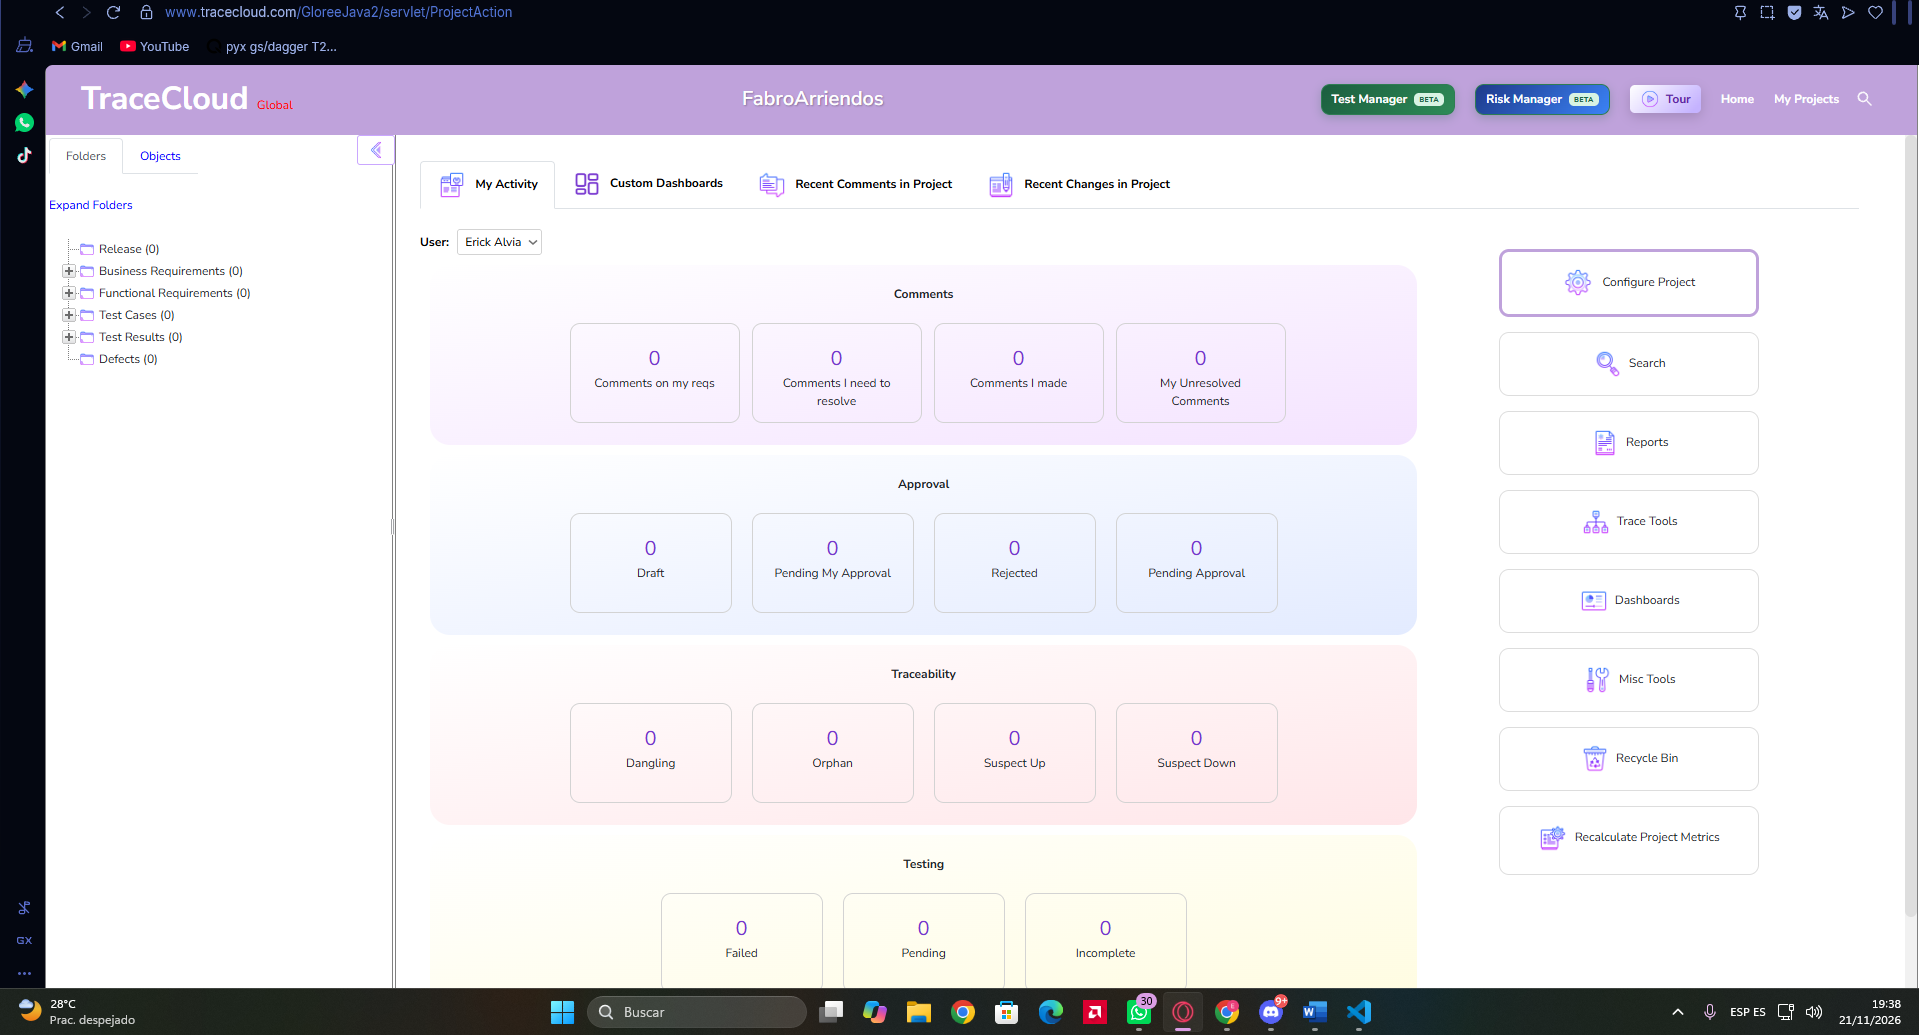
\includegraphics[width=8.65cm,height=4.18cm]{Evidencias/TraceCloud-CAP-01.png}};
\end{scope}
\path[fill=white, rounded corners=0.18cm] (9.77,2.76) rectangle (15.13,6.97);
\node[anchor=north west,inner sep=0pt,text width=4.50cm,align=left,font={\fontsize{7.17}{8.9}\selectfont\bfseries},text=accent] at (10.13,3.03) {CAPTURA 01};
\node[anchor=north west,inner sep=0pt,text width=4.50cm,align=left,font={\fontsize{5.96}{7.4}\selectfont\bfseries},text=muted] at (10.13,3.45) {EVIDENCIA DEL EQUIPO};
\fill[accent] (10.21,4.06) circle (0.07cm);
\node[anchor=north west,inner sep=0pt,text width=4.25cm,align=left,font={\fontsize{8.51}{10.6}\selectfont},text=ink] at (10.48,3.92) {Business Requirements};
\fill[accent] (10.21,4.65) circle (0.07cm);
\node[anchor=north west,inner sep=0pt,text width=4.25cm,align=left,font={\fontsize{8.51}{10.6}\selectfont},text=ink] at (10.48,4.51) {Functional Requirements};
\fill[accent] (10.21,5.24) circle (0.07cm);
\node[anchor=north west,inner sep=0pt,text width=4.25cm,align=left,font={\fontsize{8.51}{10.6}\selectfont},text=ink] at (10.48,5.10) {Test Cases};
\node[anchor=north west,inner sep=0pt,text width=8.70cm,align=left,font={\fontsize{6.70}{8.3}\selectfont},text=muted] at (0.90,7.36) {TraceCloud-CAP-01.png};
\end{scope}
\end{tikzpicture}
\note{Esta es la primera evidencia de la práctica. El equipo creó el proyecto FabroArriendos a partir de la plantilla Generic. La estructura incluye carpetas para requisitos de negocio, requisitos funcionales y casos de prueba. En el panel se observan accesos a configuración, búsqueda, reportes, herramientas de trazabilidad y tableros. Para una demostración oral conviene señalar las carpetas de la izquierda y luego abrir los requisitos registrados.}
\end{frame}

\begin{frame}[plain]
\begin{tikzpicture}[remember picture,overlay,x=1cm,y=-1cm]
\begin{scope}[shift={(current page.north west)}]
\path[use as bounding box] (0,0) rectangle (16,9);
\fill[bg] (0,0) rectangle (16,9);
\fill[accent] (0,0) rectangle (0.15,9);
\fill[wash] (15.10,0.65) circle (0.80cm);
\node[anchor=north west,inner sep=0pt,text width=12.00cm,align=left,font={\fontsize{6.37}{7.9}\selectfont\bfseries},text=accent] at (0.76,0.46) {08 / DEMOSTRACIÓN · 02};
\node[anchor=north west,inner sep=0pt,text width=14.50cm,align=left,font={\fontsize{16.42}{20.4}\selectfont\bfseries},text=ink] at (0.76,1.08) {Historias de usuario registradas};
\node[anchor=north west,inner sep=0pt,text width=14.10cm,align=left,font={\fontsize{8.17}{10.1}\selectfont},text=muted] at (0.79,1.91) {Business Requirements / Client A};
\draw[draw=linecol,line width=0.01cm] (0.77,8.48) -- (15.28,8.48);
\node[anchor=north west,inner sep=0pt,text width=7.00cm,align=left,font={\fontsize{5.16}{6.4}\selectfont\bfseries},text=muted] at (0.78,8.61) {UTEQ  /  ISR-401  /  AALM};
\node[anchor=north west,inner sep=0pt,text width=0.50cm,align=right,font={\fontsize{5.83}{7.2}\selectfont\bfseries},text=muted] at (14.82,8.60) {10};
\path[fill=linecol, rounded corners=0.12cm] (0.89,2.88) rectangle (9.54,7.06);
\path[fill=white, rounded corners=0.14cm] (0.73,2.70) rectangle (9.54,7.04);
\begin{scope}
\clip[rounded corners=0.09cm] (0.81,2.78) rectangle (9.46,6.96);
\node[anchor=north west,inner sep=0pt] at (0.81,2.78) {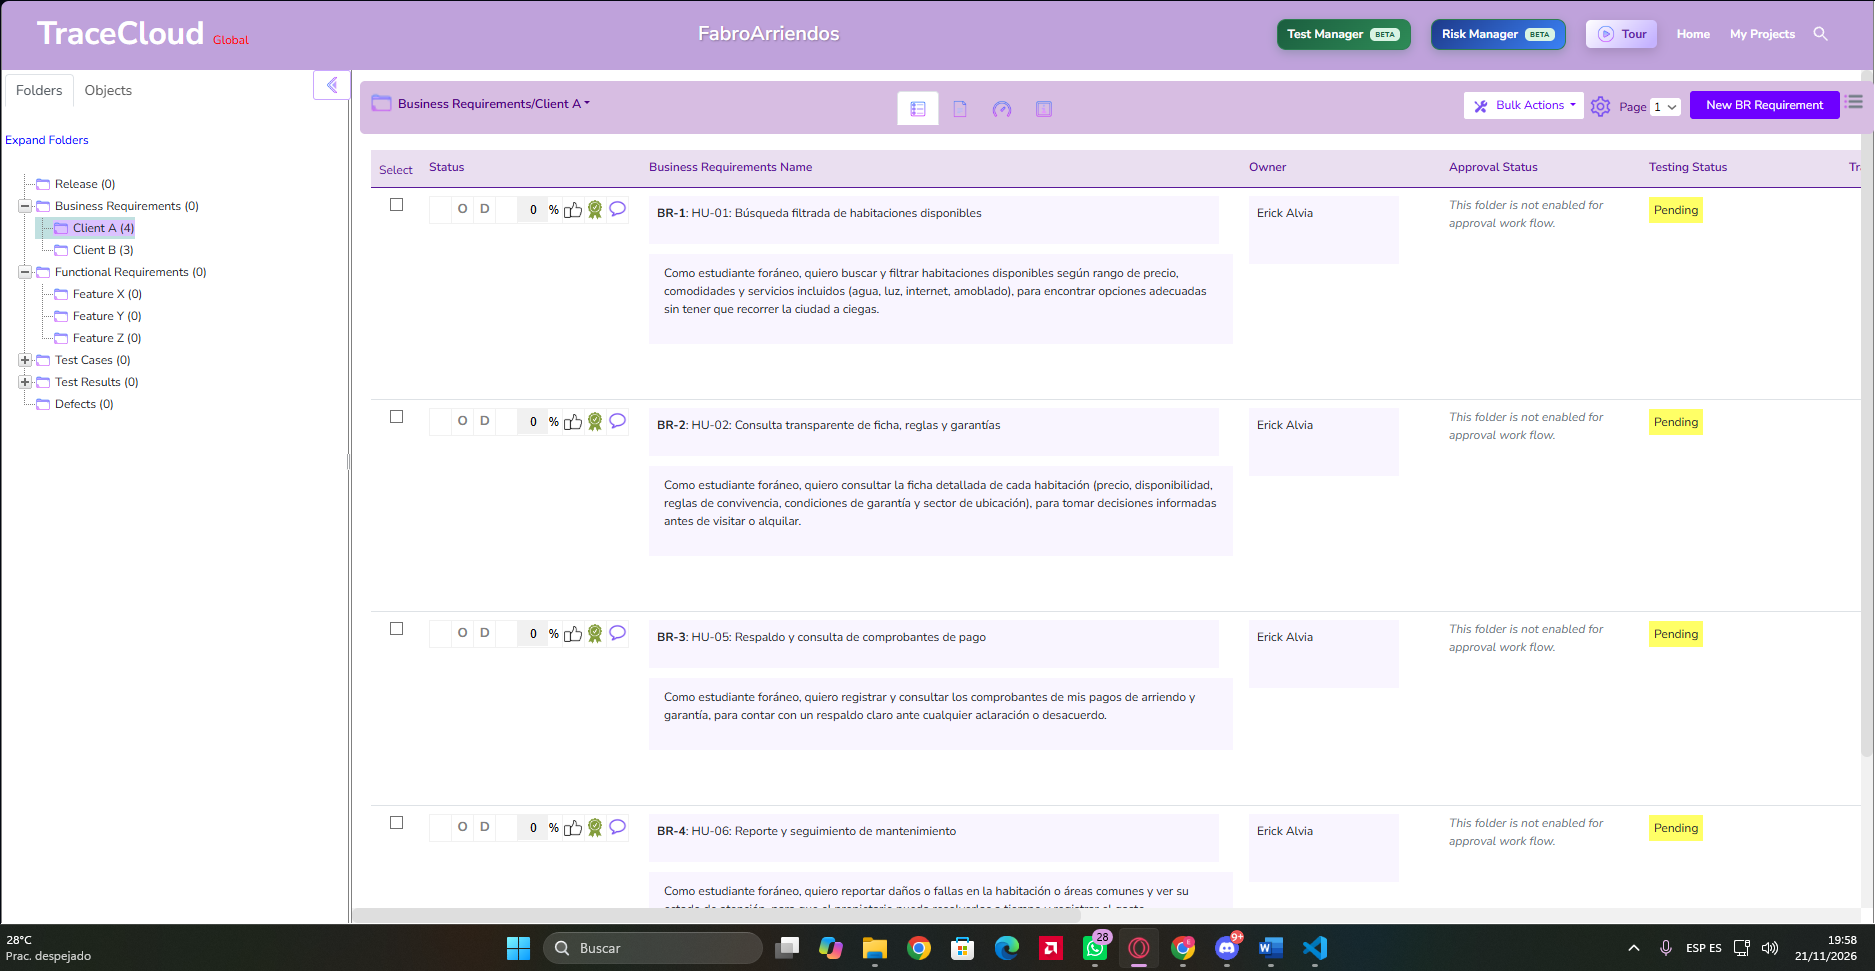
\includegraphics[width=8.65cm,height=4.18cm]{Evidencias/TraceCloud-CAP-02.png}};
\end{scope}
\path[fill=white, rounded corners=0.18cm] (9.77,2.76) rectangle (15.13,6.97);
\node[anchor=north west,inner sep=0pt,text width=4.50cm,align=left,font={\fontsize{7.17}{8.9}\selectfont\bfseries},text=accent] at (10.13,3.03) {CAPTURA 02};
\node[anchor=north west,inner sep=0pt,text width=4.50cm,align=left,font={\fontsize{5.96}{7.4}\selectfont\bfseries},text=muted] at (10.13,3.45) {EVIDENCIA DEL EQUIPO};
\fill[accent] (10.21,4.06) circle (0.07cm);
\node[anchor=north west,inner sep=0pt,text width=4.25cm,align=left,font={\fontsize{7.64}{9.5}\selectfont},text=ink] at (10.48,3.92) {BR-1  ·  Búsqueda filtrada};
\fill[accent] (10.21,4.65) circle (0.07cm);
\node[anchor=north west,inner sep=0pt,text width=4.25cm,align=left,font={\fontsize{7.64}{9.5}\selectfont},text=ink] at (10.48,4.51) {BR-2  ·  Ficha y reglas};
\fill[accent] (10.21,5.24) circle (0.07cm);
\node[anchor=north west,inner sep=0pt,text width=4.25cm,align=left,font={\fontsize{7.64}{9.5}\selectfont},text=ink] at (10.48,5.10) {BR-3  ·  Comprobantes};
\fill[accent] (10.21,5.83) circle (0.07cm);
\node[anchor=north west,inner sep=0pt,text width=4.25cm,align=left,font={\fontsize{7.64}{9.5}\selectfont},text=ink] at (10.48,5.69) {BR-4  ·  Mantenimiento};
\node[anchor=north west,inner sep=0pt,text width=8.70cm,align=left,font={\fontsize{6.70}{8.3}\selectfont},text=muted] at (0.90,7.36) {TraceCloud-CAP-02.png};
\end{scope}
\end{tikzpicture}
\note{La carpeta Business Requirements/Client A presenta cuatro historias de usuario registradas: BR-1/HU-01 sobre búsqueda filtrada; BR-2/HU-02 sobre consulta de información y condiciones de arriendo; BR-3/HU-05 acerca del respaldo de comprobantes de pago; y BR-4/HU-06 sobre reporte de daños y mantenimiento. La captura deja constancia del registro. Los nombres aparecen como historias de usuario, aunque se ubican en la estructura de requisitos de negocio de la plantilla.}
\end{frame}

\begin{frame}[plain]
\begin{tikzpicture}[remember picture,overlay,x=1cm,y=-1cm]
\begin{scope}[shift={(current page.north west)}]
\path[use as bounding box] (0,0) rectangle (16,9);
\fill[bg] (0,0) rectangle (16,9);
\fill[accent] (0,0) rectangle (0.15,9);
\fill[wash] (15.10,0.65) circle (0.80cm);
\node[anchor=north west,inner sep=0pt,text width=12.00cm,align=left,font={\fontsize{6.37}{7.9}\selectfont\bfseries},text=accent] at (0.76,0.46) {08 / DEMOSTRACIÓN · 03};
\node[anchor=north west,inner sep=0pt,text width=14.50cm,align=left,font={\fontsize{16.42}{20.4}\selectfont\bfseries},text=ink] at (0.76,1.08) {Requisitos funcionales registrados};
\node[anchor=north west,inner sep=0pt,text width=14.10cm,align=left,font={\fontsize{8.17}{10.1}\selectfont},text=muted] at (0.79,1.91) {Functional Requirements / Feature X};
\draw[draw=linecol,line width=0.01cm] (0.77,8.48) -- (15.28,8.48);
\node[anchor=north west,inner sep=0pt,text width=7.00cm,align=left,font={\fontsize{5.16}{6.4}\selectfont\bfseries},text=muted] at (0.78,8.61) {UTEQ  /  ISR-401  /  AALM};
\node[anchor=north west,inner sep=0pt,text width=0.50cm,align=right,font={\fontsize{5.83}{7.2}\selectfont\bfseries},text=muted] at (14.82,8.60) {11};
\path[fill=linecol, rounded corners=0.12cm] (0.89,2.88) rectangle (9.54,7.06);
\path[fill=white, rounded corners=0.14cm] (0.73,2.70) rectangle (9.54,7.04);
\begin{scope}
\clip[rounded corners=0.09cm] (0.81,2.78) rectangle (9.46,6.96);
\node[anchor=north west,inner sep=0pt] at (0.81,2.78) {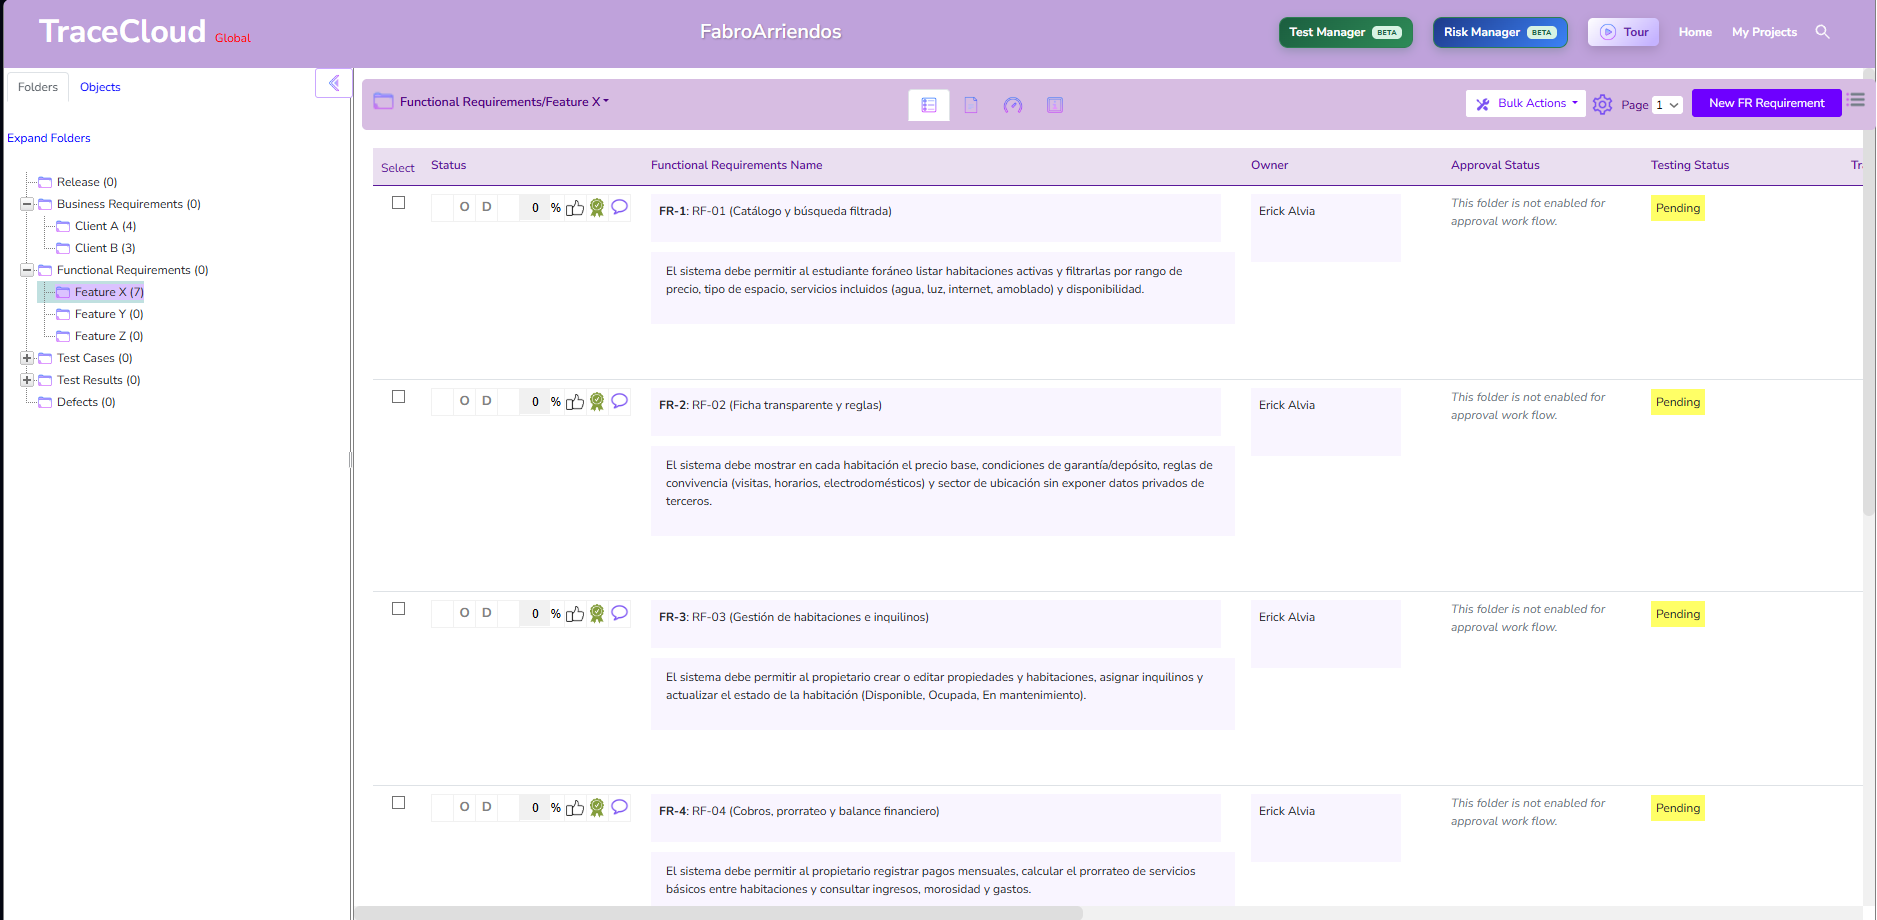
\includegraphics[width=8.65cm,height=4.18cm]{Evidencias/TraceCloud-CAP-03.png}};
\end{scope}
\path[fill=white, rounded corners=0.18cm] (9.77,2.76) rectangle (15.13,6.97);
\node[anchor=north west,inner sep=0pt,text width=4.50cm,align=left,font={\fontsize{7.17}{8.9}\selectfont\bfseries},text=accent] at (10.13,3.03) {CAPTURA 03};
\node[anchor=north west,inner sep=0pt,text width=4.50cm,align=left,font={\fontsize{5.96}{7.4}\selectfont\bfseries},text=muted] at (10.13,3.45) {EVIDENCIA DEL EQUIPO};
\fill[accent] (10.21,4.06) circle (0.07cm);
\node[anchor=north west,inner sep=0pt,text width=4.25cm,align=left,font={\fontsize{7.64}{9.5}\selectfont},text=ink] at (10.48,3.92) {FR-1  ·  Catálogo y filtros};
\fill[accent] (10.21,4.65) circle (0.07cm);
\node[anchor=north west,inner sep=0pt,text width=4.25cm,align=left,font={\fontsize{7.64}{9.5}\selectfont},text=ink] at (10.48,4.51) {FR-2  ·  Ficha transparente};
\fill[accent] (10.21,5.24) circle (0.07cm);
\node[anchor=north west,inner sep=0pt,text width=4.25cm,align=left,font={\fontsize{7.64}{9.5}\selectfont},text=ink] at (10.48,5.10) {FR-3  ·  Gestión de habitaciones};
\fill[accent] (10.21,5.83) circle (0.07cm);
\node[anchor=north west,inner sep=0pt,text width=4.25cm,align=left,font={\fontsize{7.64}{9.5}\selectfont},text=ink] at (10.48,5.69) {FR-4  ·  Cobros y balances};
\node[anchor=north west,inner sep=0pt,text width=8.70cm,align=left,font={\fontsize{6.70}{8.3}\selectfont},text=muted] at (0.90,7.36) {TraceCloud-CAP-03.png};
\end{scope}
\end{tikzpicture}
\note{En Functional Requirements/Feature X el documento registra cuatro requisitos funcionales principales, FR-1 a FR-4. FR-1 define el catálogo y la búsqueda filtrada por precio, servicios y disponibilidad; FR-2 la información detallada de cada habitación; FR-3 la administración de propiedades, habitaciones e inquilinos; FR-4 pagos, prorrateo y balance financiero. La captura presentada también muestra más elementos en la carpeta Feature X, pero la tabla detallada del informe documenta específicamente FR-1 a FR-4 como parte del ejemplo explicado. Evitar declarar que esos son todos los requisitos existentes.}
\end{frame}

\begin{frame}[plain]
\begin{tikzpicture}[remember picture,overlay,x=1cm,y=-1cm]
\begin{scope}[shift={(current page.north west)}]
\path[use as bounding box] (0,0) rectangle (16,9);
\fill[bg] (0,0) rectangle (16,9);
\fill[accent] (0,0) rectangle (0.15,9);
\fill[wash] (15.10,0.65) circle (0.80cm);
\node[anchor=north west,inner sep=0pt,text width=12.00cm,align=left,font={\fontsize{6.37}{7.9}\selectfont\bfseries},text=accent] at (0.76,0.46) {08 / DEMOSTRACIÓN · 04};
\node[anchor=north west,inner sep=0pt,text width=14.50cm,align=left,font={\fontsize{16.42}{20.4}\selectfont\bfseries},text=ink] at (0.76,1.08) {Trazabilidad de extremo a extremo};
\node[anchor=north west,inner sep=0pt,text width=14.10cm,align=left,font={\fontsize{8.17}{10.1}\selectfont},text=muted] at (0.79,1.91) {Necesidad de negocio, funcionalidad y casos de prueba.};
\draw[draw=linecol,line width=0.01cm] (0.77,8.48) -- (15.28,8.48);
\node[anchor=north west,inner sep=0pt,text width=7.00cm,align=left,font={\fontsize{5.16}{6.4}\selectfont\bfseries},text=muted] at (0.78,8.61) {UTEQ  /  ISR-401  /  AALM};
\node[anchor=north west,inner sep=0pt,text width=0.50cm,align=right,font={\fontsize{5.83}{7.2}\selectfont\bfseries},text=muted] at (14.82,8.60) {12};
\path[fill=linecol, rounded corners=0.12cm] (0.91,2.87) rectangle (9.34,7.04);
\path[fill=white, rounded corners=0.14cm] (0.75,2.69) rectangle (9.34,7.02);
\begin{scope}
\clip[rounded corners=0.09cm] (0.83,2.77) rectangle (9.26,6.94);
\node[anchor=north west,inner sep=0pt] at (0.83,2.77) {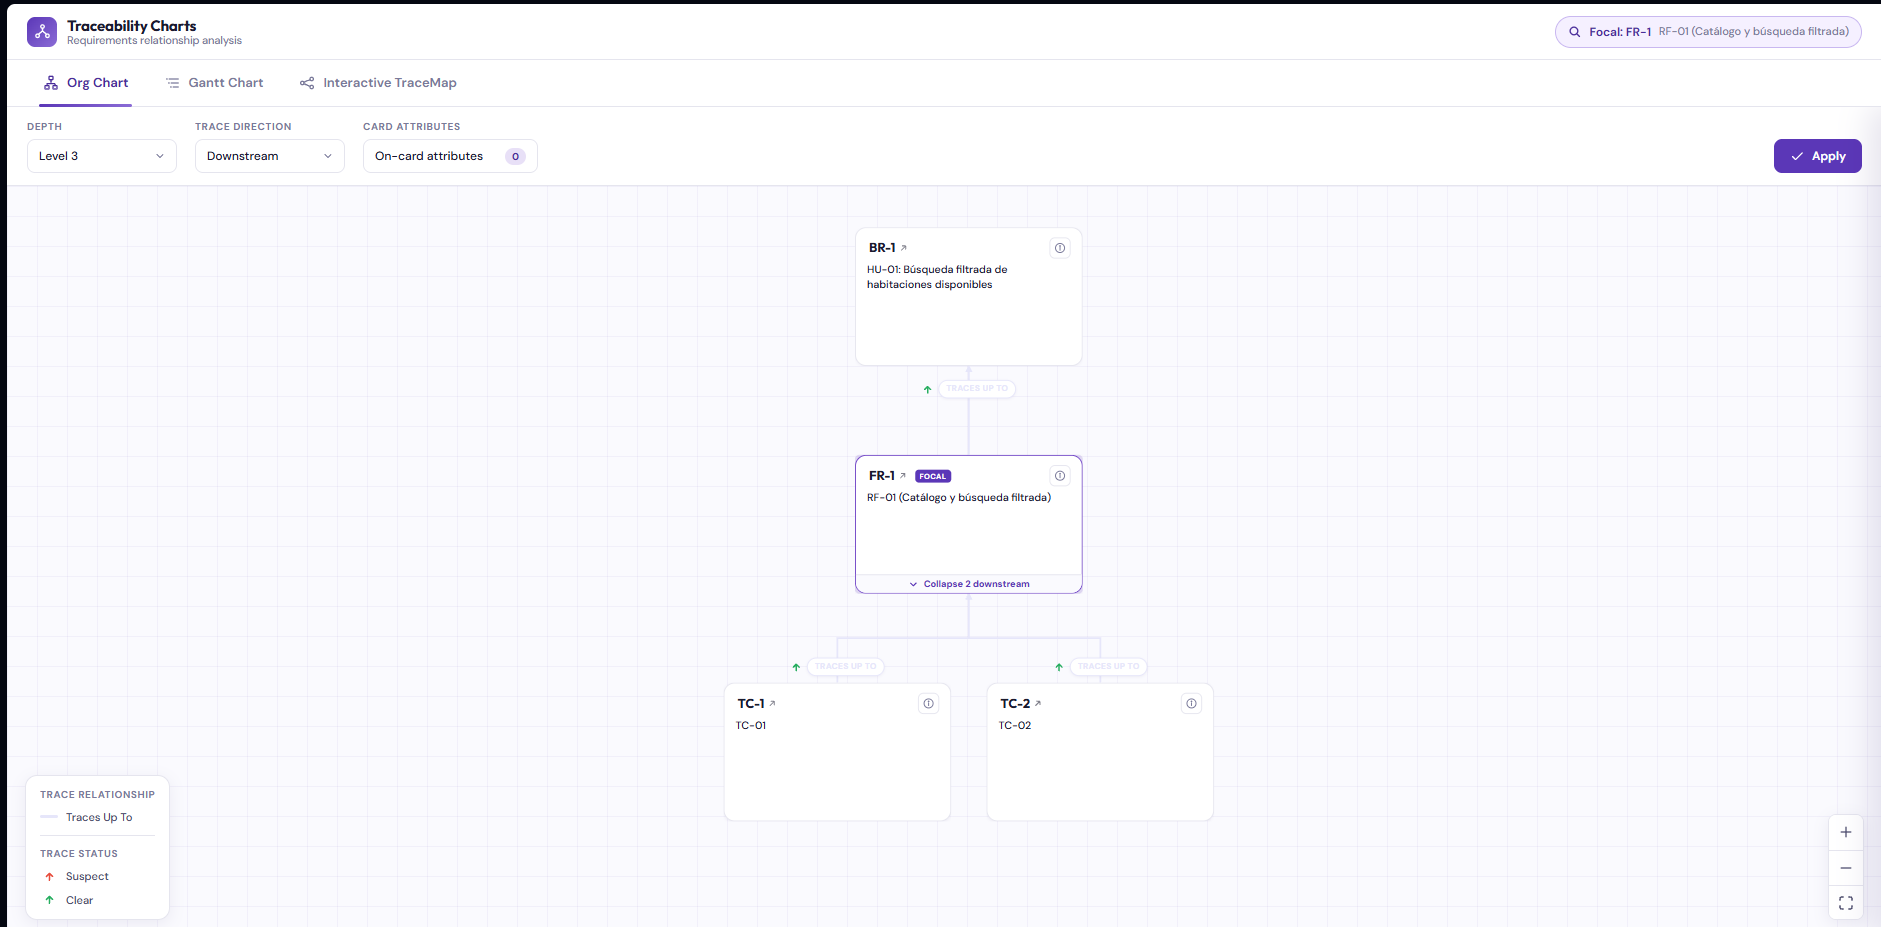
\includegraphics[width=8.43cm,height=4.17cm]{Evidencias/TraceCloud-CAP-04.png}};
\end{scope}
\path[fill=white, rounded corners=0.18cm] (9.64,2.76) rectangle (15.12,6.95);
\node[anchor=north west,inner sep=0pt,text width=4.30cm,align=left,font={\fontsize{6.97}{8.6}\selectfont\bfseries},text=accent] at (10.02,3.03) {CAPTURA 04};
\path[fill=wash, rounded corners=0.12cm] (10.15,3.53) rectangle (14.62,4.21);
\node[anchor=north west,inner sep=0pt,text width=2.55cm,align=left,font={\fontsize{8.31}{10.3}\selectfont\bfseries},text=ink] at (10.35,3.66) {BR-1 / HU-01};
\node[anchor=north west,inner sep=0pt,text width=1.42cm,align=right,font={\fontsize{6.37}{7.9}\selectfont\bfseries},text=accent] at (12.93,3.68) {Necesidad};
\draw[draw=accent,line width=0.03cm,-Latex] (12.35,4.21) -- (12.35,4.49);
\path[fill=wash, rounded corners=0.12cm] (10.15,4.51) rectangle (14.62,5.19);
\node[anchor=north west,inner sep=0pt,text width=2.55cm,align=left,font={\fontsize{8.31}{10.3}\selectfont\bfseries},text=ink] at (10.35,4.64) {FR-1 / RF-01};
\node[anchor=north west,inner sep=0pt,text width=1.42cm,align=right,font={\fontsize{6.37}{7.9}\selectfont\bfseries},text=accent] at (12.93,4.66) {Función};
\draw[draw=accent,line width=0.03cm,-Latex] (12.35,5.19) -- (12.35,5.47);
\path[fill=wash, rounded corners=0.12cm] (10.15,5.49) rectangle (14.62,6.17);
\node[anchor=north west,inner sep=0pt,text width=2.55cm,align=left,font={\fontsize{8.31}{10.3}\selectfont\bfseries},text=ink] at (10.35,5.62) {TC-1 / TC-2};
\node[anchor=north west,inner sep=0pt,text width=1.42cm,align=right,font={\fontsize{6.37}{7.9}\selectfont\bfseries},text=accent] at (12.93,5.64) {Verificación};
\node[anchor=north west,inner sep=0pt,text width=8.70cm,align=left,font={\fontsize{6.70}{8.3}\selectfont},text=muted] at (0.90,7.38) {Vista: Traceability Charts / Org Chart};
\end{scope}
\end{tikzpicture}
\note{La demostración utilizó la vista Traceability Charts, Org Chart, con FR-1 como elemento focal. El equipo estableció una relación ascendente desde FR-1/RF-01 hacia BR-1/HU-01, que describe la búsqueda filtrada de habitaciones. A su vez, FR-1 se relacionó con dos casos de prueba, TC-1 y TC-2. La captura permite visualizar el encadenamiento entre necesidad de negocio, requisito funcional y pruebas. Esta traza es el punto de partida para el ensayo de impacto de cambios.}
\end{frame}

\begin{frame}[plain]
\begin{tikzpicture}[remember picture,overlay,x=1cm,y=-1cm]
\begin{scope}[shift={(current page.north west)}]
\path[use as bounding box] (0,0) rectangle (16,9);
\fill[bg] (0,0) rectangle (16,9);
\fill[accent] (0,0) rectangle (0.15,9);
\fill[wash] (15.10,0.65) circle (0.80cm);
\node[anchor=north west,inner sep=0pt,text width=12.00cm,align=left,font={\fontsize{6.37}{7.9}\selectfont\bfseries},text=accent] at (0.76,0.46) {08 / DEMOSTRACIÓN · 05};
\node[anchor=north west,inner sep=0pt,text width=14.50cm,align=left,font={\fontsize{16.42}{20.4}\selectfont\bfseries},text=ink] at (0.76,1.08) {Cambio detectado: alerta SUSPECT};
\node[anchor=north west,inner sep=0pt,text width=14.10cm,align=left,font={\fontsize{8.17}{10.1}\selectfont},text=muted] at (0.79,1.91) {BR-1 se modificó y la relación exige nueva revisión.};
\draw[draw=linecol,line width=0.01cm] (0.77,8.48) -- (15.28,8.48);
\node[anchor=north west,inner sep=0pt,text width=7.00cm,align=left,font={\fontsize{5.16}{6.4}\selectfont\bfseries},text=muted] at (0.78,8.61) {UTEQ  /  ISR-401  /  AALM};
\node[anchor=north west,inner sep=0pt,text width=0.50cm,align=right,font={\fontsize{5.83}{7.2}\selectfont\bfseries},text=muted] at (14.82,8.60) {13};
\path[fill=linecol, rounded corners=0.12cm] (0.92,2.87) rectangle (9.54,7.04);
\path[fill=white, rounded corners=0.14cm] (0.76,2.69) rectangle (9.54,7.02);
\begin{scope}
\clip[rounded corners=0.09cm] (0.84,2.77) rectangle (9.46,6.94);
\node[anchor=north west,inner sep=0pt] at (0.84,2.77) {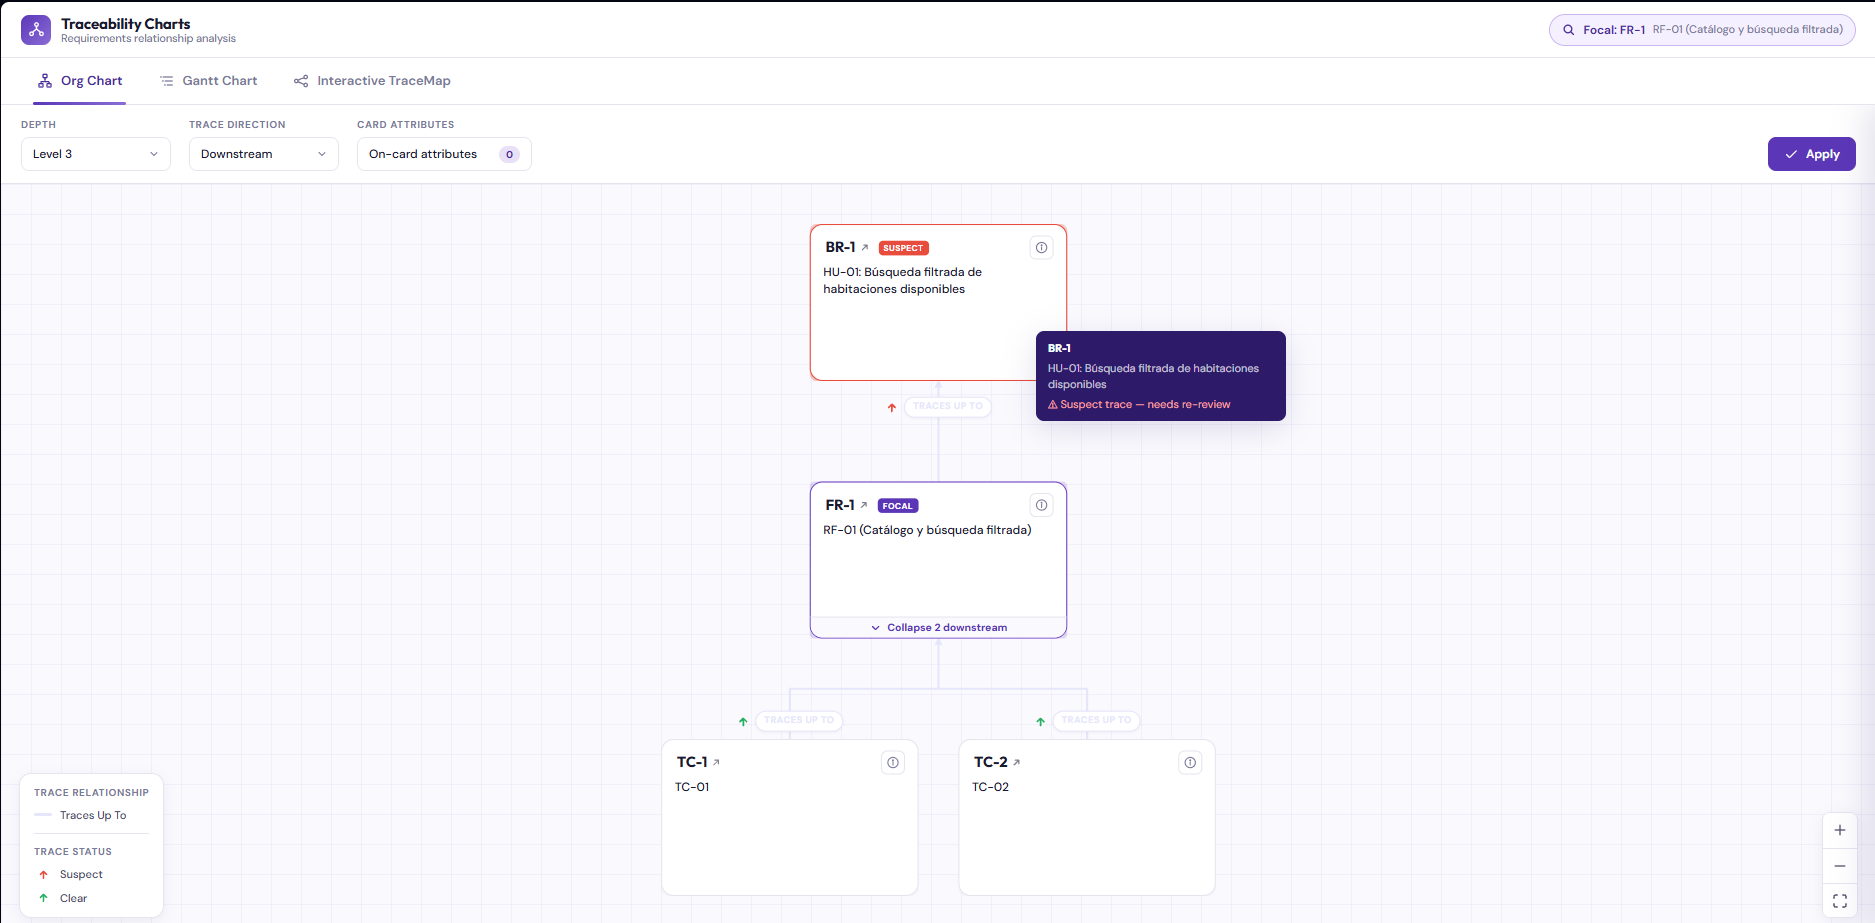
\includegraphics[width=8.62cm,height=4.17cm]{Evidencias/TraceCloud-CAP-05.png}};
\end{scope}
\path[fill=white, rounded corners=0.18cm] (9.81,2.76) rectangle (15.10,6.98);
\node[anchor=north west,inner sep=0pt,text width=4.40cm,align=left,font={\fontsize{7.04}{8.7}\selectfont\bfseries},text=accent] at (10.17,3.04) {CAPTURA 05};
\fill[accent] (10.42,3.78) circle (0.20cm);
\node[anchor=north west,inner sep=0pt,text width=0.22cm,align=center,font={\fontsize{7.37}{9.1}\selectfont\bfseries},text=white] at (10.31,3.67) {1};
\node[anchor=north west,inner sep=0pt,text width=3.79cm,align=left,font={\fontsize{8.71}{10.8}\selectfont},text=ink] at (10.84,3.65) {Edición de BR-1};
\fill[accent] (10.42,4.56) circle (0.20cm);
\node[anchor=north west,inner sep=0pt,text width=0.22cm,align=center,font={\fontsize{7.37}{9.1}\selectfont\bfseries},text=white] at (10.31,4.45) {2};
\node[anchor=north west,inner sep=0pt,text width=3.79cm,align=left,font={\fontsize{8.71}{10.8}\selectfont},text=ink] at (10.84,4.43) {Aparece alerta SUSPECT};
\fill[accent] (10.42,5.34) circle (0.20cm);
\node[anchor=north west,inner sep=0pt,text width=0.22cm,align=center,font={\fontsize{7.37}{9.1}\selectfont\bfseries},text=white] at (10.31,5.23) {3};
\node[anchor=north west,inner sep=0pt,text width=3.79cm,align=left,font={\fontsize{8.71}{10.8}\selectfont},text=ink] at (10.84,5.21) {El equipo debe revalidar};
\path[fill=wash, rounded corners=0.08cm] (10.17,6.33) rectangle (14.73,6.76);
\node[anchor=north west,inner sep=0pt,text width=4.20cm,align=center,font={\fontsize{7.10}{8.8}\selectfont\bfseries},text=accent] at (10.32,6.43) {ALERTA  ≠  VALIDACIÓN};
\node[anchor=north west,inner sep=0pt,text width=8.70cm,align=left,font={\fontsize{6.70}{8.3}\selectfont},text=muted] at (0.90,7.36) {TraceCloud-CAP-05.png};
\end{scope}
\end{tikzpicture}
\note{Para comprobar el análisis de impacto, el equipo editó la descripción de BR-1/HU-01. TraceCloud indicó visualmente una condición SUSPECT y el mensaje “Suspect trace — needs re-review” en el vínculo mostrado. El resultado demuestra la detección de una relación que necesita revisión; no demuestra que el sistema sepa automáticamente cómo corregirla ni que el requisito actualizado haya sido revalidado. El analista debe evaluar si los requisitos y pruebas vinculados siguen siendo coherentes. Esta es la evidencia más importante de la exposición.}
\end{frame}

\begin{frame}[plain]
\begin{tikzpicture}[remember picture,overlay,x=1cm,y=-1cm]
\begin{scope}[shift={(current page.north west)}]
\path[use as bounding box] (0,0) rectangle (16,9);
\fill[bg] (0,0) rectangle (16,9);
\fill[accent] (0,0) rectangle (0.15,9);
\fill[wash] (15.10,0.65) circle (0.80cm);
\node[anchor=north west,inner sep=0pt,text width=12.00cm,align=left,font={\fontsize{6.37}{7.9}\selectfont\bfseries},text=accent] at (0.76,0.46) {09 / SÍNTESIS};
\node[anchor=north west,inner sep=0pt,text width=14.50cm,align=left,font={\fontsize{16.42}{20.4}\selectfont\bfseries},text=ink] at (0.76,1.08) {¿Qué demuestra el caso práctico?};
\node[anchor=north west,inner sep=0pt,text width=14.10cm,align=left,font={\fontsize{8.17}{10.1}\selectfont},text=muted] at (0.79,1.91) {Resultados observados, límites y transparencia metodológica [6], [8].};
\draw[draw=linecol,line width=0.01cm] (0.77,8.48) -- (15.28,8.48);
\node[anchor=north west,inner sep=0pt,text width=7.00cm,align=left,font={\fontsize{5.16}{6.4}\selectfont\bfseries},text=muted] at (0.78,8.61) {UTEQ  /  ISR-401  /  AALM};
\node[anchor=north west,inner sep=0pt,text width=0.50cm,align=right,font={\fontsize{5.83}{7.2}\selectfont\bfseries},text=muted] at (14.82,8.60) {14};
\path[fill=wash, rounded corners=0.19cm] (0.85,2.78) rectangle (7.79,6.55);
\node[anchor=north west,inner sep=0pt,text width=5.77cm,align=left,font={\fontsize{8.31}{10.3}\selectfont\bfseries},text=teal] at (1.34,3.20) {APORTES};
\fill[teal] (1.38,4.17) circle (0.11cm);
\node[anchor=north west,inner sep=0pt,text width=5.75cm,align=left,font={\fontsize{9.18}{11.4}\selectfont},text=ink] at (1.71,4.02) {Centralización de requisitos};
\fill[teal] (1.38,4.86) circle (0.11cm);
\node[anchor=north west,inner sep=0pt,text width=5.75cm,align=left,font={\fontsize{9.18}{11.4}\selectfont},text=ink] at (1.71,4.71) {Trazas entre BR, FR y TC};
\fill[teal] (1.38,5.55) circle (0.11cm);
\node[anchor=north west,inner sep=0pt,text width=5.75cm,align=left,font={\fontsize{9.18}{11.4}\selectfont},text=ink] at (1.71,5.40) {Detección de cambios vinculados};
\path[fill=white, rounded corners=0.19cm] (8.12,2.78) rectangle (15.06,6.55);
\node[anchor=north west,inner sep=0pt,text width=5.77cm,align=left,font={\fontsize{8.31}{10.3}\selectfont\bfseries},text=accent] at (8.61,3.20) {LÍMITES};
\fill[accent] (8.65,4.17) circle (0.11cm);
\node[anchor=north west,inner sep=0pt,text width=5.75cm,align=left,font={\fontsize{9.18}{11.4}\selectfont},text=ink] at (8.98,4.02) {No reemplaza entrevistas};
\fill[accent] (8.65,4.86) circle (0.11cm);
\node[anchor=north west,inner sep=0pt,text width=5.75cm,align=left,font={\fontsize{9.18}{11.4}\selectfont},text=ink] at (8.98,4.71) {Revisión humana necesaria};
\fill[accent] (8.65,5.55) circle (0.11cm);
\node[anchor=north west,inner sep=0pt,text width=5.75cm,align=left,font={\fontsize{9.18}{11.4}\selectfont},text=ink] at (8.98,5.40) {ReqIF no confirmado};
\path[fill=white, rounded corners=0.14cm] (0.90,6.72) rectangle (15.10,7.24);
\node[anchor=north west,inner sep=0pt,text width=13.50cm,align=center,font={\fontsize{8.40}{10.8}\selectfont\bfseries},text=accent] at (1.18,6.87) {La alerta detecta revisión pendiente; no valida automáticamente la traza [8].};
\path[fill=wash, rounded corners=0.12cm] (0.90,7.35) rectangle (15.10,8.19);
\node[anchor=north west,inner sep=0pt,text width=13.30cm,align=left,font={\fontsize{6.65}{8.6}\selectfont\bfseries},text=accent] at (1.18,7.49) {DECLARACIÓN DE IA (apoyo editorial, no evidencia de campo)};
\node[anchor=north west,inner sep=0pt,text width=13.40cm,align=left,font={\fontsize{6.10}{7.9}\selectfont},text=ink] at (1.18,7.79) {Claude Sonnet 3.5; ChatGPT GPT-4o y GPT-6; Gemini (versión por confirmar). Verificación: fuentes, capturas y compilación; responsabilidad del equipo.};
\end{scope}
\end{tikzpicture}
\note{Declaración de herramientas: el informe de origen declara Claude Sonnet 3.5 para estructura y corrección de LaTeX; ChatGPT GPT-4o y Gemini para revisión de texto, figuras y coherencia. En esta revisión adicional se empleó ChatGPT GPT-6 para edición técnica, bibliografía, reproducibilidad y diseño. La versión concreta de Gemini no consta en el material recibido, por lo que debe confirmarla el equipo antes de la entrega; no se atribuye a IA la generación de entrevistas o capturas originales. Las salidas se validan mediante contraste bibliográfico, revisión visual de capturas y dos ejecuciones de pdflatex. Los integrantes deben verificar la veracidad de la declaración. Conclusión del estudio: TraceCloud aporta mecanismos para centralizar y controlar los requisitos, vincular necesidades con funcionalidades y casos de prueba, y advertir relaciones que requieren revisión tras un cambio. En Fabro Arriendos el equipo verificó una alerta Suspect después de editar BR-1, lo que ilustra su utilidad para el análisis de impacto. Sin embargo, TraceCloud no sustituye las técnicas cualitativas de elicitación ni la responsabilidad del equipo en validar los vínculos. Además, la documentación consultada no permite asegurar compatibilidad con ReqIF. Cierre oral: una herramienta automatiza parte del control, no reemplaza el análisis de requisitos.}
\end{frame}

\begin{frame}[plain]
\begin{tikzpicture}[remember picture,overlay,x=1cm,y=-1cm]
\begin{scope}[shift={(current page.north west)}]
\path[use as bounding box] (0,0) rectangle (16,9);
\fill[bg] (0,0) rectangle (16,9);
\fill[accent] (0,0) rectangle (0.15,9);
\fill[wash] (15.10,0.65) circle (0.80cm);
\node[anchor=north west,inner sep=0pt,text width=12.00cm,align=left,font={\fontsize{6.37}{7.9}\selectfont\bfseries},text=accent] at (0.76,0.46) {10 / RESPALDO ACADÉMICO};
\node[anchor=north west,inner sep=0pt,text width=14.50cm,align=left,font={\fontsize{16.42}{20.4}\selectfont\bfseries},text=ink] at (0.76,1.08) {Referencias bibliográficas};
\node[anchor=north west,inner sep=0pt,text width=14.10cm,align=left,font={\fontsize{8.17}{10.1}\selectfont},text=muted] at (0.79,1.91) {Fuentes originales del informe · Referencias [1]--[4].};
\draw[draw=linecol,line width=0.01cm] (0.77,8.48) -- (15.28,8.48);
\node[anchor=north west,inner sep=0pt,text width=7.00cm,align=left,font={\fontsize{5.16}{6.4}\selectfont\bfseries},text=muted] at (0.78,8.61) {UTEQ / ISR-401 / AALM};
\node[anchor=north west,inner sep=0pt,text width=0.50cm,align=right,font={\fontsize{5.83}{7.2}\selectfont\bfseries},text=muted] at (14.82,8.60) {15};
\path[fill=white, rounded corners=0.15cm] (0.86,2.55) rectangle (15.15,3.79);
\path[fill=wash, rounded corners=0.10cm] (1.03,2.73) rectangle (1.62,3.26);
\node[anchor=north west,inner sep=0pt,text width=0.53cm,align=center,font={\fontsize{8.2}{10.3}\selectfont\bfseries},text=accent] at (1.06,2.85) {[1]};
\node[anchor=north west,inner sep=0pt,text width=12.98cm,align=left,font={\fontsize{7.90}{10.74}\selectfont},text=ink] at (1.77,2.71) {K. Pohl, \emph{Requirements Engineering: Fundamentals, Principles, and Techniques}, 2.\textsuperscript{a} ed., Berlin--Heidelberg: Springer, 2025. ISBN: 978-3-662-69204-2.};
\path[fill=white, rounded corners=0.15cm] (0.86,3.91) rectangle (15.15,5.15);
\path[fill=wash, rounded corners=0.10cm] (1.03,4.09) rectangle (1.62,4.62);
\node[anchor=north west,inner sep=0pt,text width=0.53cm,align=center,font={\fontsize{8.2}{10.3}\selectfont\bfseries},text=accent] at (1.06,4.21) {[2]};
\node[anchor=north west,inner sep=0pt,text width=12.98cm,align=left,font={\fontsize{7.20}{9.70}\selectfont},text=ink] at (1.77,4.07) {S. Bühne, M. Glinz, H. van Loenhoud y S. Staal, \emph{IREB Certified Professional for Requirements Engineering --- Foundation Level Syllabus}, versión 3.3.0, IREB e.V., Karlsruhe, Alemania, 1 abr. 2026.};
\path[fill=white, rounded corners=0.15cm] (0.86,5.27) rectangle (15.15,6.51);
\path[fill=wash, rounded corners=0.10cm] (1.03,5.45) rectangle (1.62,5.98);
\node[anchor=north west,inner sep=0pt,text width=0.53cm,align=center,font={\fontsize{8.2}{10.3}\selectfont\bfseries},text=accent] at (1.06,5.57) {[3]};
\node[anchor=north west,inner sep=0pt,text width=12.98cm,align=left,font={\fontsize{7.90}{10.74}\selectfont},text=ink] at (1.77,5.43) {H. Washizaki (ed.), \emph{Guide to the Software Engineering Body of Knowledge (SWEBOK Guide)}, versión 4.0, Los Alamitos, California: IEEE Computer Society, 2024.};
\path[fill=white, rounded corners=0.15cm] (0.86,6.63) rectangle (15.15,8.07);
\path[fill=wash, rounded corners=0.10cm] (1.03,6.81) rectangle (1.62,7.34);
\node[anchor=north west,inner sep=0pt,text width=0.53cm,align=center,font={\fontsize{8.2}{10.3}\selectfont\bfseries},text=accent] at (1.06,6.93) {[4]};
\node[anchor=north west,inner sep=0pt,text width=12.98cm,align=left,font={\fontsize{7.90}{10.74}\selectfont},text=ink] at (1.77,6.79) {H. Cheng et al., ``Generative AI for requirements engineering: A systematic literature review'', \emph{Software: Practice and Experience}, vol. 56, n.º 2, pp. 141--170, 2026. DOI: \href{https://doi.org/10.1002/spe.70029}{10.1002/spe.70029}.};
\end{scope}
\end{tikzpicture}
\note{Corrección bibliográfica [2] contrastada con la portada oficial del syllabus IREB 3.3.0, donde constan cuatro autores: Stan Bühne, Martin Glinz, Hans van Loenhoud y Stefan Staal. Referencias completas [1] a [4] según el archivo referencias.bib del informe. Incluyen los fundamentos de ingeniería de requisitos, el programa IREB, SWEBOK 4.0 y el estudio sobre IA generativa en requisitos.}
\end{frame}

\begin{frame}[plain]
\begin{tikzpicture}[remember picture,overlay,x=1cm,y=-1cm]
\begin{scope}[shift={(current page.north west)}]
\path[use as bounding box] (0,0) rectangle (16,9);
\fill[bg] (0,0) rectangle (16,9);
\fill[accent] (0,0) rectangle (0.15,9);
\fill[wash] (15.10,0.65) circle (0.80cm);
\node[anchor=north west,inner sep=0pt,text width=12.00cm,align=left,font={\fontsize{6.37}{7.9}\selectfont\bfseries},text=accent] at (0.76,0.46) {10 / RESPALDO ACADÉMICO};
\node[anchor=north west,inner sep=0pt,text width=14.50cm,align=left,font={\fontsize{16.42}{20.4}\selectfont\bfseries},text=ink] at (0.76,1.08) {Referencias bibliográficas};
\node[anchor=north west,inner sep=0pt,text width=14.10cm,align=left,font={\fontsize{8.17}{10.1}\selectfont},text=muted] at (0.79,1.91) {Fuentes originales del informe · Referencias [5]--[8].};
\draw[draw=linecol,line width=0.01cm] (0.77,8.48) -- (15.28,8.48);
\node[anchor=north west,inner sep=0pt,text width=7.00cm,align=left,font={\fontsize{5.16}{6.4}\selectfont\bfseries},text=muted] at (0.78,8.61) {UTEQ / ISR-401 / AALM};
\node[anchor=north west,inner sep=0pt,text width=0.50cm,align=right,font={\fontsize{5.83}{7.2}\selectfont\bfseries},text=muted] at (14.82,8.60) {16};
\path[fill=white, rounded corners=0.15cm] (0.86,2.47) rectangle (15.15,3.62);
\path[fill=wash, rounded corners=0.10cm] (1.03,2.65) rectangle (1.62,3.18);
\node[anchor=north west,inner sep=0pt,text width=0.53cm,align=center,font={\fontsize{8.2}{10.3}\selectfont\bfseries},text=accent] at (1.06,2.77) {[5]};
\node[anchor=north west,inner sep=0pt,text width=12.98cm,align=left,font={\fontsize{7.65}{10.40}\selectfont},text=ink] at (1.77,2.63) {A. Stein, A. Mirzai, J. Axmann y T. Vietor, ``Integrating the capabilities offered by large language models into the requirements engineering process'', \emph{Digital Engineering}, vol. 10, art. 100098, 2026. DOI: \href{https://doi.org/10.1016/j.dte.2026.100098}{10.1016/j.dte.2026.100098}.};
\path[fill=white, rounded corners=0.15cm] (0.86,3.73) rectangle (15.15,4.88);
\path[fill=wash, rounded corners=0.10cm] (1.03,3.91) rectangle (1.62,4.44);
\node[anchor=north west,inner sep=0pt,text width=0.53cm,align=center,font={\fontsize{8.2}{10.3}\selectfont\bfseries},text=accent] at (1.06,4.03) {[6]};
\node[anchor=north west,inner sep=0pt,text width=12.98cm,align=left,font={\fontsize{7.75}{10.54}\selectfont},text=ink] at (1.77,3.89) {M. Ozkaya, G. Kardas y M. A. Kose, ``An Analysis of the Features of Requirements Engineering Tools'', \emph{Systems}, vol. 11, n.º 12, art. 576, 2023. DOI: \href{https://doi.org/10.3390/systems11120576}{10.3390/systems11120576}.};
\path[fill=white, rounded corners=0.15cm] (0.86,4.99) rectangle (15.15,6.73);
\path[fill=wash, rounded corners=0.10cm] (1.03,5.17) rectangle (1.62,5.70);
\node[anchor=north west,inner sep=0pt,text width=0.53cm,align=center,font={\fontsize{8.2}{10.3}\selectfont\bfseries},text=accent] at (1.06,5.29) {[7]};
\node[anchor=north west,inner sep=0pt,text width=12.98cm,align=left,font={\fontsize{7.35}{10.00}\selectfont},text=ink] at (1.77,5.15) {A. Rozenberga y M. Kirikova, ``Enterprise Model for Requirements Management: Evaluation of Capability Gaps in Jira and Marketplace Applications'', en \emph{PoEM 2025: Companion Proceedings of the 18th IFIP Working Conference on the Practice of Enterprise Modeling}, CEUR Workshop Proceedings, vol. 4171, art. 69, 2025 (publicado en línea el 20 feb. 2026). Disponible en: \href{https://ceur-ws.org/Vol-4171/paper_69.pdf}{https://ceur-ws.org/Vol-4171/paper\_69.pdf}. Consultado: 21 nov. 2026.};
\path[fill=white, rounded corners=0.15cm] (0.86,6.84) rectangle (15.15,8.16);
\path[fill=wash, rounded corners=0.10cm] (1.03,7.02) rectangle (1.62,7.55);
\node[anchor=north west,inner sep=0pt,text width=0.53cm,align=center,font={\fontsize{8.2}{10.3}\selectfont\bfseries},text=accent] at (1.06,7.14) {[8]};
\node[anchor=north west,inner sep=0pt,text width=12.98cm,align=left,font={\fontsize{7.55}{10.27}\selectfont},text=ink] at (1.77,7.00) {J. Priya, \emph{Managing Requirements \& Improving Quality: Project Requirements Management \& Traceability}, TraceCloud, documento técnico (white paper), dic. 2020. Disponible en: \href{https://www.tracecloud.com/GloreeJava2/documentation/whitePaperTraceCloud.pdf}{https://www.tracecloud.com/GloreeJava2/documentation/whitePaperTraceCloud.pdf}. Consultado: 20 nov. 2026.};
\end{scope}
\end{tikzpicture}
\note{Referencias completas [5] a [8] conforme a referencias.bib. La referencia [7] aporta la evaluación independiente de Jira y las aplicaciones de su Marketplace, y la [8] documenta las funciones de TraceCloud. Los DOI y enlaces están incorporados como hipervínculos.}
\end{frame}

\end{document}
